\documentclass[10pt]{beamer}

\usetheme[progressbar=frametitle]{metropolis}
\usepackage{appendixnumberbeamer}

\usepackage{booktabs}
\usepackage[scale=2]{ccicons}
\usepackage{multimedia}
\usepackage{wrapfig}
\usepackage{tabularx}
\usepackage{esint}
\usepackage{amsmath}
\usepackage{pgfplots}
\usepgfplotslibrary{dateplot}
\usepackage{fancybox}
\usepackage{xspace}
\newcommand{\themename}{\textbf{\textsc{metropolis}}\xspace}

\setsansfont[BoldFont={Fira Sans}]{Fira Sans Light}
\setmonofont{Fira Mono}

%\usepackage[bold-style=ISO]{unicode-math}                    
%\setmathfont{Latin Modern Math}
%\setmathfont[range={\mathscr,\mathbfscr}]{XITS Math}

\title{Flight control of a Quadrotor Vehicle Subsequent to a	Rotor Failure}
\date{}
\author{Edoardo Ghini, Gianluca Cerilli, Giuseppe L'Erario}
\institute{Modeling and control of multi-rotor UAVs}
\titlegraphic{\hfill
\includegraphics[height=1.0cm]{Images/SapienzaLogo.pdf}}

\begin{document}
	
	\maketitle
	
\begin{frame}{Table of contents}
	\setbeamertemplate{section in toc}[sections numbered]
	\tableofcontents[hideallsubsections]
\end{frame}

\section{Introduction}

\begin{frame}{Problem statement}

Development of a control scheme in case of \textbf{rotor failure}, to allow the quadrotor to land with only three actuators.

\end{frame}

\begin{frame}{Proposed Strategy}

\textbf{Full control of attitude is lost}: renounce the yaw angle control, maintaining flight control of a spinning vehicle\\
\bigskip
\textbf{Double-loop architecture}\\
\begin{list}{$ \circ $}{}
	\item \textit{Outer Control}\\
	Yaw velocity is computed instead of the yaw angle\\
	\bigskip
	\item \textit{Inner Control}\\
	Roll angle, pitch angle and yaw velocity regulated via feedback linearization
\end{list}

\end{frame}

\section{Quadrotor Model}

\begin{frame}{Control Model}

\begin{columns}
\begin{column}{0.3\textwidth}
\begin{itemize}
	\item Symmetric
	\bigskip
	\item Rigid propellers
	\bigskip
	\item Linear drag
\end{itemize}
\end{column}
\begin{column}{0.7\textwidth}
\begin{figure}
	\centering
	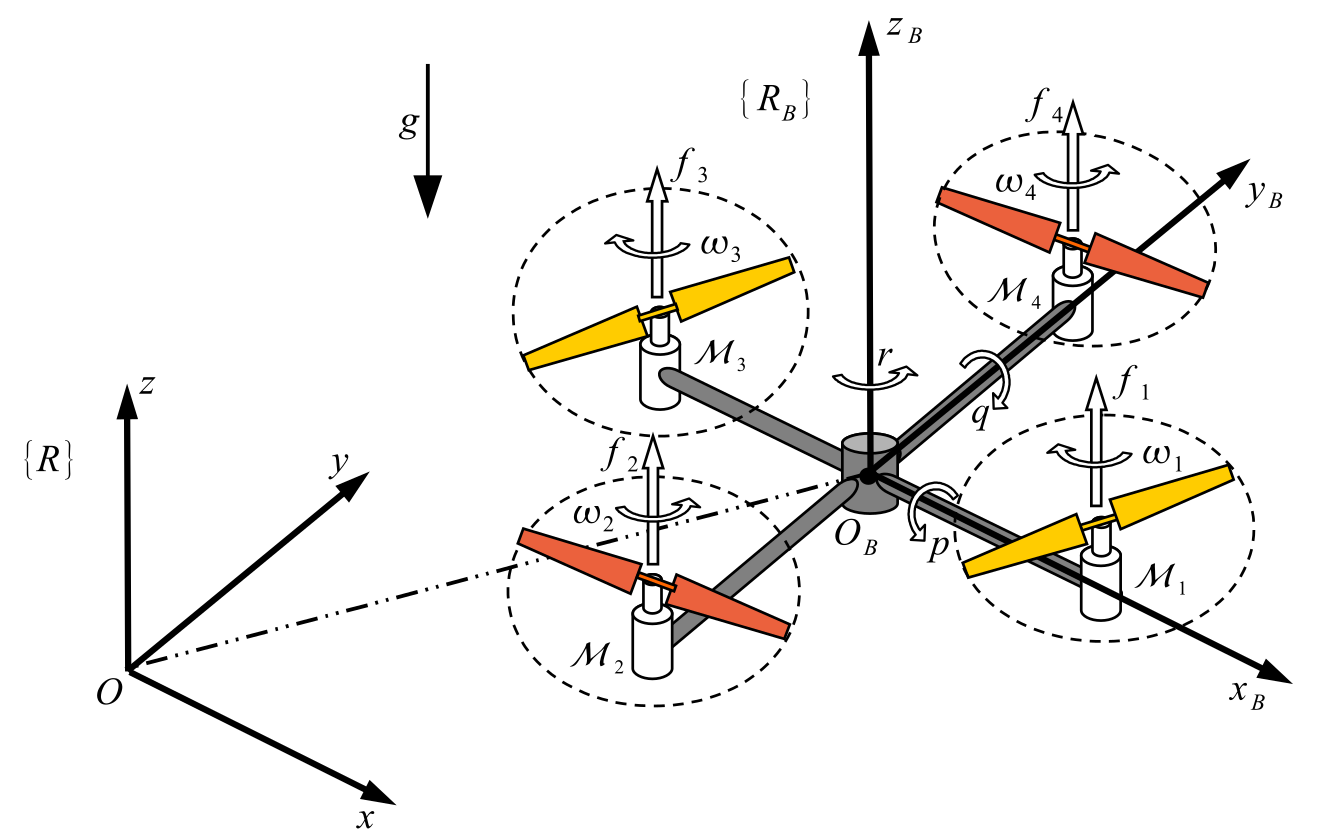
\includegraphics[width=0.9\linewidth]{Images/Quad_model}
\end{figure}
\end{column}
\end{columns}
Two reference frames:\\
\bigskip
\begin{itemize}
\item Earth frame: $ \{R\}\{O, x, y, z\} $
\item Body-fixed frame: $ \{R_b\}\{O_b, x_b, y_b, z_b\} $
\end{itemize}

\end{frame}

\begin{frame}{Control Model}

\textbf{Rotations} along roll ($ \phi $) and pitch ($ \theta $) angles are constrained:
\begin{equation*}
(-\frac{\Pi}{2}<\phi<\frac{\Pi}{2}), \qquad (-\frac{\Pi}{2}<\theta<\frac{\Pi}{2})
\end{equation*}
while yaw angle $ \psi $ is unconstrained.\\
\bigskip
\textbf{Inertia matrix} in the body frame:
\begin{equation*}
\mathbf{I}=
\begin{bmatrix}
I_{xx} & 0 & 0 \\
0 & I_{yy} & 0 \\
0 & 0 & I_{zz} 
\end{bmatrix}
\end{equation*}
where $ I_{xx} = I_{yy} $ due to symmetry.

\end{frame}

\begin{frame}{Control Model}

\textbf{Dynamic model}, defined from generalized forces, drag force and weight:
\begin{equation*}
\begin{cases}
\ddot{x} = \frac{1}{m}[(C_{\phi}S_{\theta}C_{\psi} + S_{\phi}S_{\psi})u_f-k_t \dot{x}] \\
\ddot{y} = \frac{1}{m}[(C_{\phi}S_{\theta}S_{\psi} - S_{\phi}C_{\psi})u_f-k_t \dot{y}] \\
\ddot{z} = \frac{1}{m}[(C_{\phi}C_{\theta})u_f- mg - k_t \dot{z}] \\
\dot{p} = \frac{1}{I_{xx}}[-k_r p - qr(I_{zz}-I_{yy})+\tau_p]  \\
\dot{q} = \frac{1}{I_{yy}}[-k_r q - pr(I_{xx}-I_{zz})+\tau_q]  \\
\dot{r} = \frac{1}{I_{zz}}[-k_r r - pq(I_{yy}-I_{xx})+\tau_r]  \\
\dot{\phi} = p + q S_{\phi}T_{\theta} + r C_{\phi}T_{\theta} \\
\dot{\theta} = q C_{\phi} - rS_{\phi} \\
\dot{\psi} = \frac{1}{C_{\theta}}[qS_{\phi}+rC_{\phi}]
\end{cases}
\end{equation*}

\begin{itemize}
\item $ k_r, k_t $ = rotational and linear drags, $ N \cdot m \cdot s  $;
\item $ u_f $ = total upward lift force, $ N $;
\item $ \tau_p, \ \tau_q, \ \tau_r $ = torque around roll, pitch and yaw axis, $ N\cdot m $;
\end{itemize}

\end{frame}

\begin{frame}{Control Model}
\textbf{System inputs}:\\ Generalized forces $ u_f, \ \tau_p, \ \tau_q, \ \tau_r $\\
\bigskip 
\textbf{Real actuation}:\\
Four motors forces $ f_1, \ f_2, \ f_3, \ f_4 $\\
\bigskip
Relation between these is given by:
\begin{equation}
\begin{bmatrix}
u_f \\ \tau_p \\ \tau_q \\ \tau_r
\end{bmatrix} = 
\begin{bmatrix}
1 & 1 & 1 & 1 \\
0 & -l & 0 & l \\
-l & 0 & l & 0 \\
d & -d & d & -d
\end{bmatrix}
\begin{bmatrix}
f_1 \\ f_2 \\ f_3 \\ f_4
\end{bmatrix}
\label{force_mapping}
\end{equation}
where
\begin{itemize}
\item \textit{d} = ratio between drag and thrust coefficient of the rotor, $ m $
\item \textit{l} = arm length, $ m $
\end{itemize}

\end{frame}

\section*{Introduction}

%This work deals with the development of a controller able to suppress the vibration and unwanted inputs in a bilateral control system.

Teleoperation extends the human capability to manipulating objects remotely. An important aspect deals with necessity to obtain, on operator side, similar condition as those at the remote location, in other words, a proper feedback. 

A bilateral system is composed by a joystick, called \emph{master}, on the human side, connected to a \emph{slave} on the environment side.

The human imposes a force on the master, that results in a displacement. This displacement is then transmitted to the slave. On the other side, the slave has a force sensor used to "send back" to the master the reflection forces at the environment side. For these reasons we can call it \emph{bilateral teleoperation}.

Two important goals of the teleoperation are \cite{hokayem2006bilateral}:
\begin{itemize}
	\item \textbf{Stability} of the closed loop system irrespective to the behavior of the human and the environment;
	\item \textbf{Transparency} of the teleoperation task: we want forces and displacements be the same on the two sides of the system. 
\end{itemize}

Stability of the system can be ruined by unwanted disturbance, internal and external:
\begin{itemize}
	\item \textbf{Internal disturbance}, due to the uncertainties in modeling of the system;
	\item \textbf{External disturbance}, such as unexpected input contaminated with vibration noise from both sides og the system.
\end{itemize}

This report deals with the development of a controller able to suppress the vibration and unwanted inputs in a bilateral control system \cite{trakarnchaiyo2017vibration}.

In particular, the work is based on the concept of one degree of freedom inertia-spring-damper system. This concept comes from the design of shock absorbers used in vehicle suspension (which is composed by a spring and damper), and is usually applied in bilateral control system for \emph{soft manipulation}.

In this work we investigate the concept of \textit{virtual} spring-damper system with an additional inertia.
The disturbance suppression performances depends on the value of these virtual parameters, determined from the desired cut-off frequencies.

The report is organized as follow: in the first part we model the inertia-spring-damper system, analyzing the proposed control and the hybrid matrix. Then is the described the virtual parameter selection process. Finally, we present the results obtained in the simulations, performed with Matlab and Simulink.

\section{System Modeling}

\subsection*{Nomenclature}

\begin{itemize}
	\item $ J_m $ = inertia of the master, $ \text{kg m}^2 $;
	\item $ J_s $ = inertia of the slave,  $ \text{kg m}^2 $;
	\item $ J_{mv} $ = virtual inertia of the master,  $ \text{kg m}^2 $;
	\item $ J_{sv} $ = virtual inertia of the slave,  $ \text{kg m}^2 $;
	\item $ B_v $ = virtual damping of the system, $ \frac{\text{N m}}{\text{rad/s}} $;
	\item $ K_v $ = virtual spring of the system, $ \frac{\text{N m}}{\text{rad}} $;
	\item $ \tau_m $ = master torque, $ \text{N m} $;
	\item $ \theta_m $ = master displacement, $ \text{rad} $; 
	\item $ \tau_s $ = slave torque, $ \text{N m} $;
	\item $ \theta_s $ = slave displacement, $ \text{rad} $;
\end{itemize}

\subsection{Modeling}

\begin{figure}[h]
	\centering
	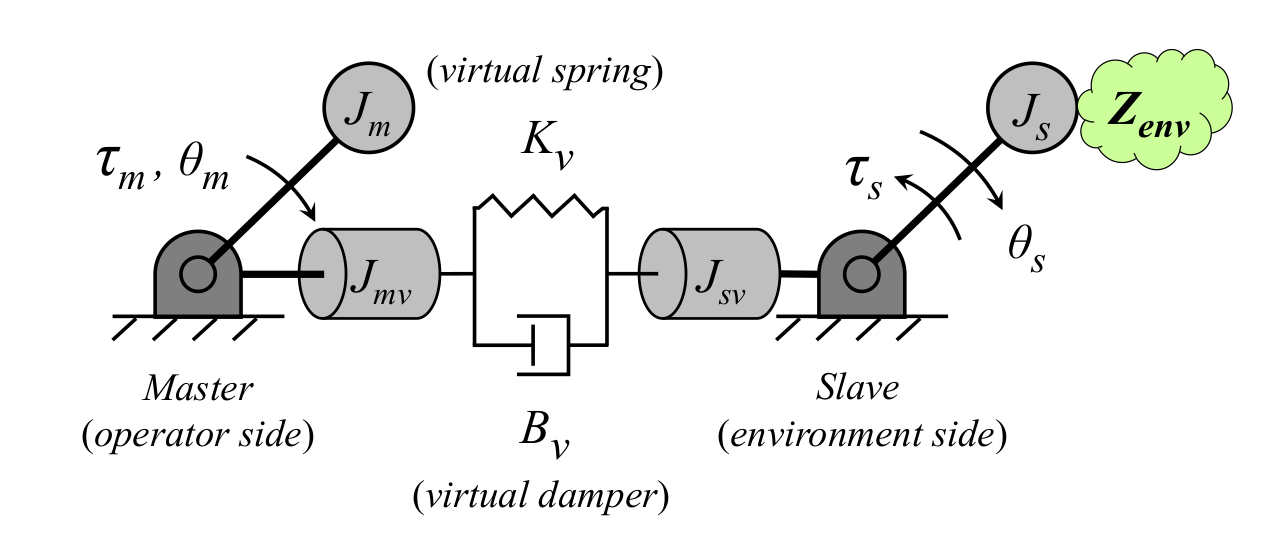
\includegraphics[width=0.7\linewidth]{Images/spring_damper_inertia_system}
	\caption{Spring-damper-inertia system with virtual parameters.}
	\label{fig:springdamperinertiasystem}
\end{figure}


The inertia-spring-damping system is shown in Fig.\ref{fig:springdamperinertiasystem}: the master and the slave have the real inertia $ J_m $ and $ J_s $ and the virtual ones $ J_{mv} $ and $ J_{sv} $. Master and slave are interconnected with the virtual damper $ B_v $ and the virtual spring $ K_v $.

The dynamic equation of the system are:
\begin{align}
	(J_m + J_{mv})\ddot{\theta}_m + B_v (\dot{\theta}_m - \dot{\theta}_s) + K_v(\theta_m - \theta_s) &= \tau_m \\
	(J_s + J_{sv})\ddot{\theta}_s + B_v (\dot{\theta}_s - \dot{\theta}_m) + K_v(\theta_s - \theta_m) &= - \tau_s 
\end{align}
and, in frequency domain:
\begin{align}
	(J_m + J_{mv}) s^2 \theta_m + (B_v s + K_v) (\theta_m - \theta_s) &= \tau_m \\
	(J_s + J_{sv}) s^2 \theta_s + (B_v s + K_v) (\theta_s - \theta_m) &= - \tau_s 
\end{align}

The virtual parameters are considered elements of the controller. For this aim the equations above are rearranged:
\begin{align}
	J_m s^2 \theta_m &= \tau_m - (B_v s + K_v) (\theta_m - \theta_s) - J_{mv} s^2 \theta_m \\
	J_s s^2 \theta_s &= - \tau_s - (B_v s + K_v) (\theta_s - \theta_m) - J_{sv} s^2 \theta_s \\
\end{align}
where the external torques are action and reaction forces of the human and the environment.

The block diagram of the proposed control system is constructed as shown in Fig.\ref{fig:blockdiagram}\footnote{Delay time in communication channel is not considered in the reference paper \cite{trakarnchaiyo2017vibration}.}.

\begin{figure}
	\centering
	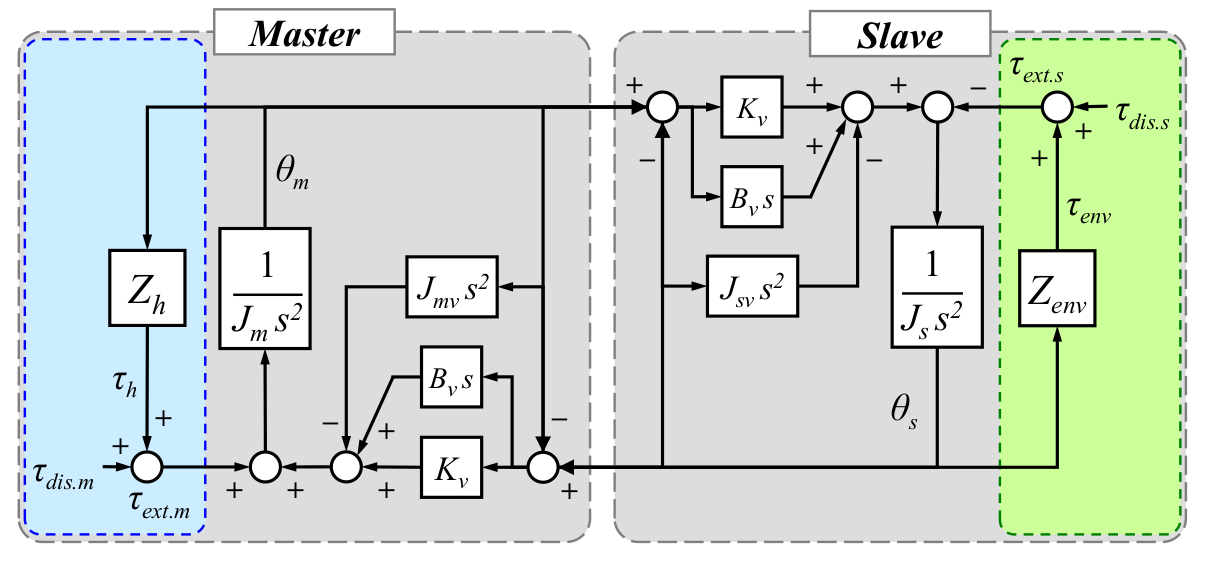
\includegraphics[width=0.7\linewidth]{Images/Block_diagram}
	\caption[block_diagram]{Block diagram of the bilateral control system.}
	\label{fig:blockdiagram}
\end{figure}

A bilateral control can be represented by a 2x2 matrix, called \emph{hybrid matrix}:
\begin{equation}
	\begin{bmatrix}
	\tau_m \\ \theta_s
	\end{bmatrix} = 
	\begin{bmatrix}
	H_{11} & H_{12} \\
	H_{21} & H_{22}
	\end{bmatrix}
	\begin{bmatrix}
	\theta_m \\ - \tau_s
	\end{bmatrix}
	\label{hybrid_matrix}
\end{equation}
and every $ H_{ij} $ is an hybrid parameter.

In particular:
\begin{align}
	H_{11} &= \frac{1}{Z_s}[Z_m Z_s - (B_v s + K_v)^2] \\
	H_{12} &= -\frac{1}{Z_s}[B_v s + K_v] \\
	H_{21} &= \frac{1}{Z_s}[B_v s + K_v] \\
	H_{22} &= \frac{1}{Z_s} 
\end{align}
where:
\begin{align}
	Z_m &= (J_m + J_{mv}) s^2 + B_v s + K_v \\
	Z_s &= (J_s + J_{sv}) s^2 + B_v s + K_v
\end{align}

The system should achieve two conditions:
\begin{itemize}
	\item the position of both sides should be the same;
	\item the law of action-reaction should hold;
\end{itemize}
represented by the \emph{transparency condition}:
\begin{align}
	\tau_m = \tau_s \\
	\theta_m = \theta_s
\end{align}
is expressed in terms of transmitted impedance $ Z_t $, which is transferred to the human, and environment impedance $ Z_{env} $:
\begin{equation}
	\frac{\tau_m}{\theta_m} = Z_t = Z_{env} = \frac{\tau_s}{\theta_s}
	\label{transparencY_condition}
\end{equation}

The relationship between the transmitted and environment impedance comes from the hybrid matrix of \eqref{hybrid_matrix}:
\begin{equation}
	Z_t = \big(\dfrac{-H_{12} H_{21}}{1 + H_{22} Z_{env}}\big)Z_{env} + H_{11}
\end{equation}
and, to achieve the perfect transparency condition shown in \eqref{transparencY_condition}, the hybrid parameters should be derived as:
\begin{equation}
	\begin{bmatrix}
	\tau_m \\ \theta_s
	\end{bmatrix} = 
	\begin{bmatrix}
	0 & -1 \\ 1 & 0
	\end{bmatrix}
	\begin{bmatrix}
	\theta_m \\ -\tau_s
	\end{bmatrix}
\end{equation}

The performances of a teleoperation are evaluated in \emph{free} and \emph{contact} motion. For free motion the external torque on the slave is usually equal to zero, and hence the only parameters affecting the transparency are $ H_{11} $ and $ H_{21} $. For contact motion, instead, all the hybrid parameters affect the performance.

\subsection{Parameter selection and design}\label{ParamSelect} 

The system is assumed to be disturbed by external vibration noise from the environment. We want to know how the slave position is affected by the external noise. This analysis can be achieved inspecting the hybrid parameter $ H_{22} $, representing how the slave position responds to external torque:
\begin{equation}
	\dfrac{\theta_s}{\tau_{ext}} = \dfrac{1}{(J_s + J_{sv}) s^2 + B_v s + K_v}
	\label{H_22}
\end{equation}

The virtual parameter in \eqref{H_22} are determined from the second-order characteristic equation of the system:
\begin{equation}
%	s^2 + (g_1 + g_2) s + (g_1 \cdot g_2) = 0
	(s + g_1)(s + g_2) = 0
	\label{charact_equation}
\end{equation}  
where the poles $ g_1 $ and $ g_2 $ represent the cut-off frequencies of the system for disturbance suppression purpose.

We can determine the virtual parameters comparing the characteristic equation of \eqref{H_22} with \eqref{charact_equation}.

The operator should feel the reflecting force from the environment vividly. Assuming for a moment we do not care about the vibration suppression, for the proposed control the system can achieve a large transparency with high spring stiffness $ K_v $ and a damping $ B_v \rightarrow 0 $. 

It is clear that the value of spring stiffness $ K_v $ has an important influence on the transparency of the system: we want to choose it beforehand and the other virtual parameters will be calculated accordingly.
The virtual damping coefficient $ B_v $:
\begin{equation}
	\frac{B_v}{K_v} = \frac{g_1 + g_2}{g_1 \cdot g_2} \quad \Rightarrow \quad B_v = \frac{g_1 + g_2}{g_1 \cdot g_2} K_v
\end{equation}
and, in the same fashion, the virtual inertia $ J_{sv} $:
\begin{equation}
	J_{sv} = \frac{1}{g_1 \cdot g_2} K_v - J_s
\end{equation}

The spring stiffness, as said before, influences the behavior of the system. Choosing it properly we can obtain:
\begin{itemize}
	\item \textbf{rigid coupling}, with high stiff spring, obtaining an high transparency;
	\item \textbf{spring coupling}, when the value of the stiffness is low.
\end{itemize}

In other words we can use the spring stiffness to regulate the \emph{compliance} of the system.

\bigskip
\section{Simulations}

\subsection{Chosen parameters}

In regards of the simulation scenarios we are deliberately neglecting the
critical aspects of the communication between master and slave.

Therefore all the following simulations has been run assuming ideal conditions as an
instantaneous and loss-less signal transfer between master and slave subsystems.

\bigskip

\begin{table}[H]
\centering
	\begin{tabular}{c c c c}
		\toprule
		Symbol & Parameter & Value & Unit\\
		\midrule 
		\midrule 
    & \textsl{Master-Slave system}\\
		\midrule 
		$J_{m}$  & Master Inertia & $5\cdot 10^{-4}$ & $\text{kg}\cdot \text{m\textsuperscript{2}}$ \\
		$J_{s}$  & Slave Inertia & $5\cdot 10^{-4}$ & $\text{kg}\cdot \text{m\textsuperscript{2}}$ \\
    \midrule 
    & \textsl{Desired cut-off frequencies}\\
		\midrule 
		$g_{1}$  & 1\textsuperscript{st} cut-off frequency & $5\cdot 10^{1}$ & rad/s \\
		$g_{2}$  & 2\textsuperscript{nd} cut-off frequency & $5\cdot 10^{2}$ & rad/s \\
		\bottomrule
	\end{tabular}
	\caption{Parameters adopted in simulations.}
	\label{simParams}
\end{table}

\bigskip

The table n.\ref{simParams} describes the parameters chosen such as inertiae and
cut-off frequencies, consequently the table n.\ref{virtParams} describes
the virtual coefficients computed as explained in section \ref{ParamSelect}.

\bigskip

\begin{table}[H]
\centering
	\begin{tabular}{c c c c}
		\toprule
		Behaviour & $K_{v}$ & $B_{v}$ &  $J_{v}$\\
		\midrule 
		\midrule 
	    Virtual compliance& $20.0 \ \frac{\text{N m}}{\text{rad}} $ & $4.4\cdot 10^{-1} \ \frac{\text{N m}}{\text{rad/s}}$ & $3\cdot 10^{-4} \ \text{kg m\textsuperscript{2}}$\\
    	Rigid coupling & $10^{2} \ \frac{\text{N m}}{\text{rad}} $ & $1.5\cdot 10^{-1} \ \frac{\text{N m}}{\text{rad/s}}$ & $ 0 \ \text{kg m\textsuperscript{2}} $\\
		\bottomrule
	\end{tabular}
	\caption{Sets of chosen virtual parameters.}
	\label{virtParams}
\end{table}
\newpage

\subsection{Disturbance rejection performances}

We consider at first the rigid coupling case, in which, as being said, almost
full transparency is achieved between master and slave. The vibrations
transmitted by the environment on the slave-side will be felt almost with the same intensity on the master-side whatever would be the vibration frequency.

\begin{figure}[h]
	\centering
	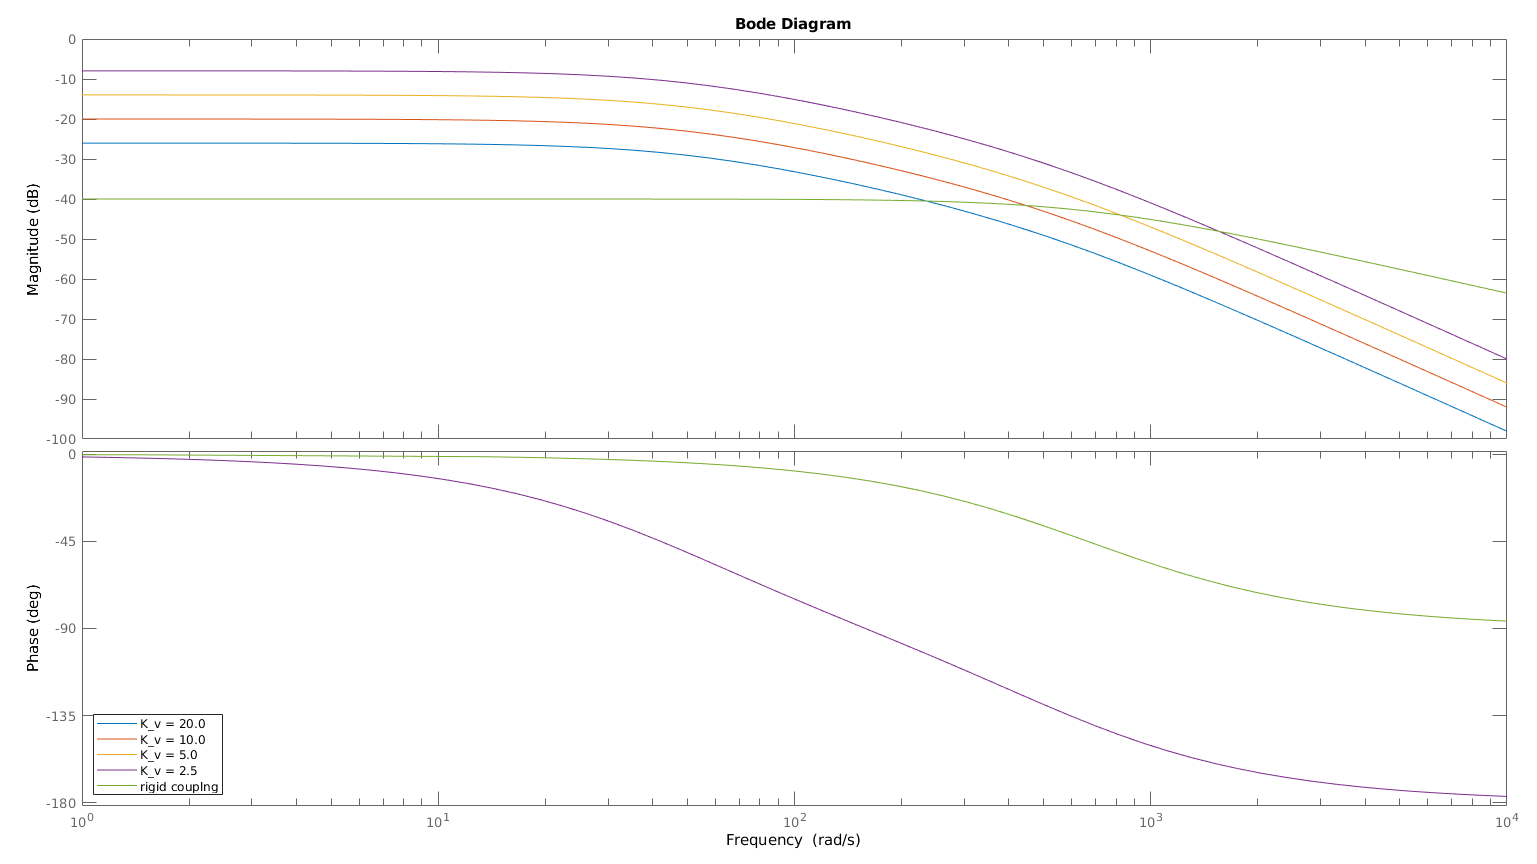
\includegraphics[width=1\linewidth]{Images/bodo}
	\caption{Frequency response relative to $ H_{22} $ hybrid parameter.}
	\label{fig:bodo}
\end{figure}

For this reason, in order to reach better task execution performances we want to
reduce the impact of environment vibrations at minimum.

The simulations aims to compare two opposite behaviours: \textbf{rigid coupling}
and \textbf{induced virtual compliance}, achieved through the choice of
the desired cut-off frequencies.

Fig.\ref{fig:bodo} describes the frequency response of the function \eqref{H_22} with several virtual parameters sets, defined starting from different spring stiffness values $ K_v $ varying from $ 2.5 \ \text{N}\cdot\text{m}/\text{rad} $ to $ 20 \ \text{N}\cdot\text{m}/\text{rad} $, and the rigid coupling control set.

At low frequencies the signals are preserved in both the rigid coupling and the virtual compliance controls. In particular, the magnitude of the response increases with inverse of the virtual spring stiffness, describing the \textbf{compliance} of the system. At high frequencies the disturbance rejection is exerted more effectively by the virtual compliance control: the position response to high frequency external torque is reduced due to the low compliance.

%This could be accomplished, as shown before, by building an ad-hoc filter, such
%as fig.\ref{fig:bodo} depicits, in which there are different slope profiles that
%will end up rejecting the disturbances at higher frequencies than the
%\textsl{cut-off} ones and preserving the signal at lower ones.

%The simulations aims to compare two opposite behaviours: \textbf{rigid coupling}
%and \textbf{induced virtual compliance} which is achieved through the choice of
%the desired cut-off frequencies.
%\newline

%Another description of the frequency response of the system is provided by the figs.\ref{positionResponceFrequencies}

%In particular these frequencies correspond respectively to 8 and 80 Hz.
A comparison of the vibration suppression applied on three
different input frequencies is interesting, (figs.\ref{positionResponceFrequencies})
\footnote{For the sake of simplicity the different control set are called:
	\begin{itemize}
		\item Control set 1 : defined by $ K_v = 20.0 \ \frac{\text{N} \cdot \text{m}}{\text{rad}}$;
		\item Control set 2 : defined by $ K_v = 10.0 \ \frac{\text{N} \cdot \text{m}}{\text{rad}}$;
		\item Control set 3 : defined by $ K_v = 5.0 \ \frac{\text{N} \cdot \text{m}}{\text{rad}}$;
		\item Control set 4 : defined by $ K_v = 2.5 \ \frac{\text{N} \cdot \text{m}}{\text{rad}}$.	
\end{itemize}
}:

\begin{itemize}
%\item $10^{1} Hz$ : In fig.\ref{fig:10Htz} is shown how the vibrations at lower frequencies are preserved by the\textsl{virtual compliance}, this is a rather enticing aspect of a teleoperation interaction since the input commands generated by the controller will have kind of low frequencies.
\item $ 10 \ \text{Hz} $ input : in fig.\ref{fig:10Htz} is shown how the inputs at lower frequencies are preserved by the \textbf{control set 4} (defined by $ K_v = 2.5 \ \text{N}\cdot\text{m/s} $ - purple line). The response is less large as stiffness increases. The phase is almost the same for virtual compliance and rigid coupling controls;
%\item $10^{2} \text{Hz}$ : The fig.\ref{fig:100Htz} demonstrates a turning point in which the disturbance rejection achieved by the \textsl{rigid coupling} is comparable to the performance of \textsl{virtual compliance}.
\item $10^{2} \ \text{Hz}$ input : as before, the response decreases as the virtual spring stiffness increase. The difference here is the almost the same response of the \textbf{control set 1} ($ K_v = 20 \ \text{N}\cdot\text{m/s} $ - blue line) and the rigid coupling ($ K_v = 10^2 \ \text{N}\cdot\text{m/s} $ - green line), despite the second one is defined by a larger value of stiffness. The phase relative to the \textbf{control sets} is delayed respect to the rigid coupling control (fig.\ref{fig:100Htz});
\item $10^{3} \ \text{Hz}$ input : at frequencies higher than the cut-off ones, the
inputs are dumped more effectively by the \textbf{control sets} than the \textbf{rigid coupling control}, for which we have larger response (fig.\ref{fig:1000Htz}).
\end{itemize}

\begin{figure}[H]
	\begin{subfigure}[h!]{1\linewidth}
		\centering
		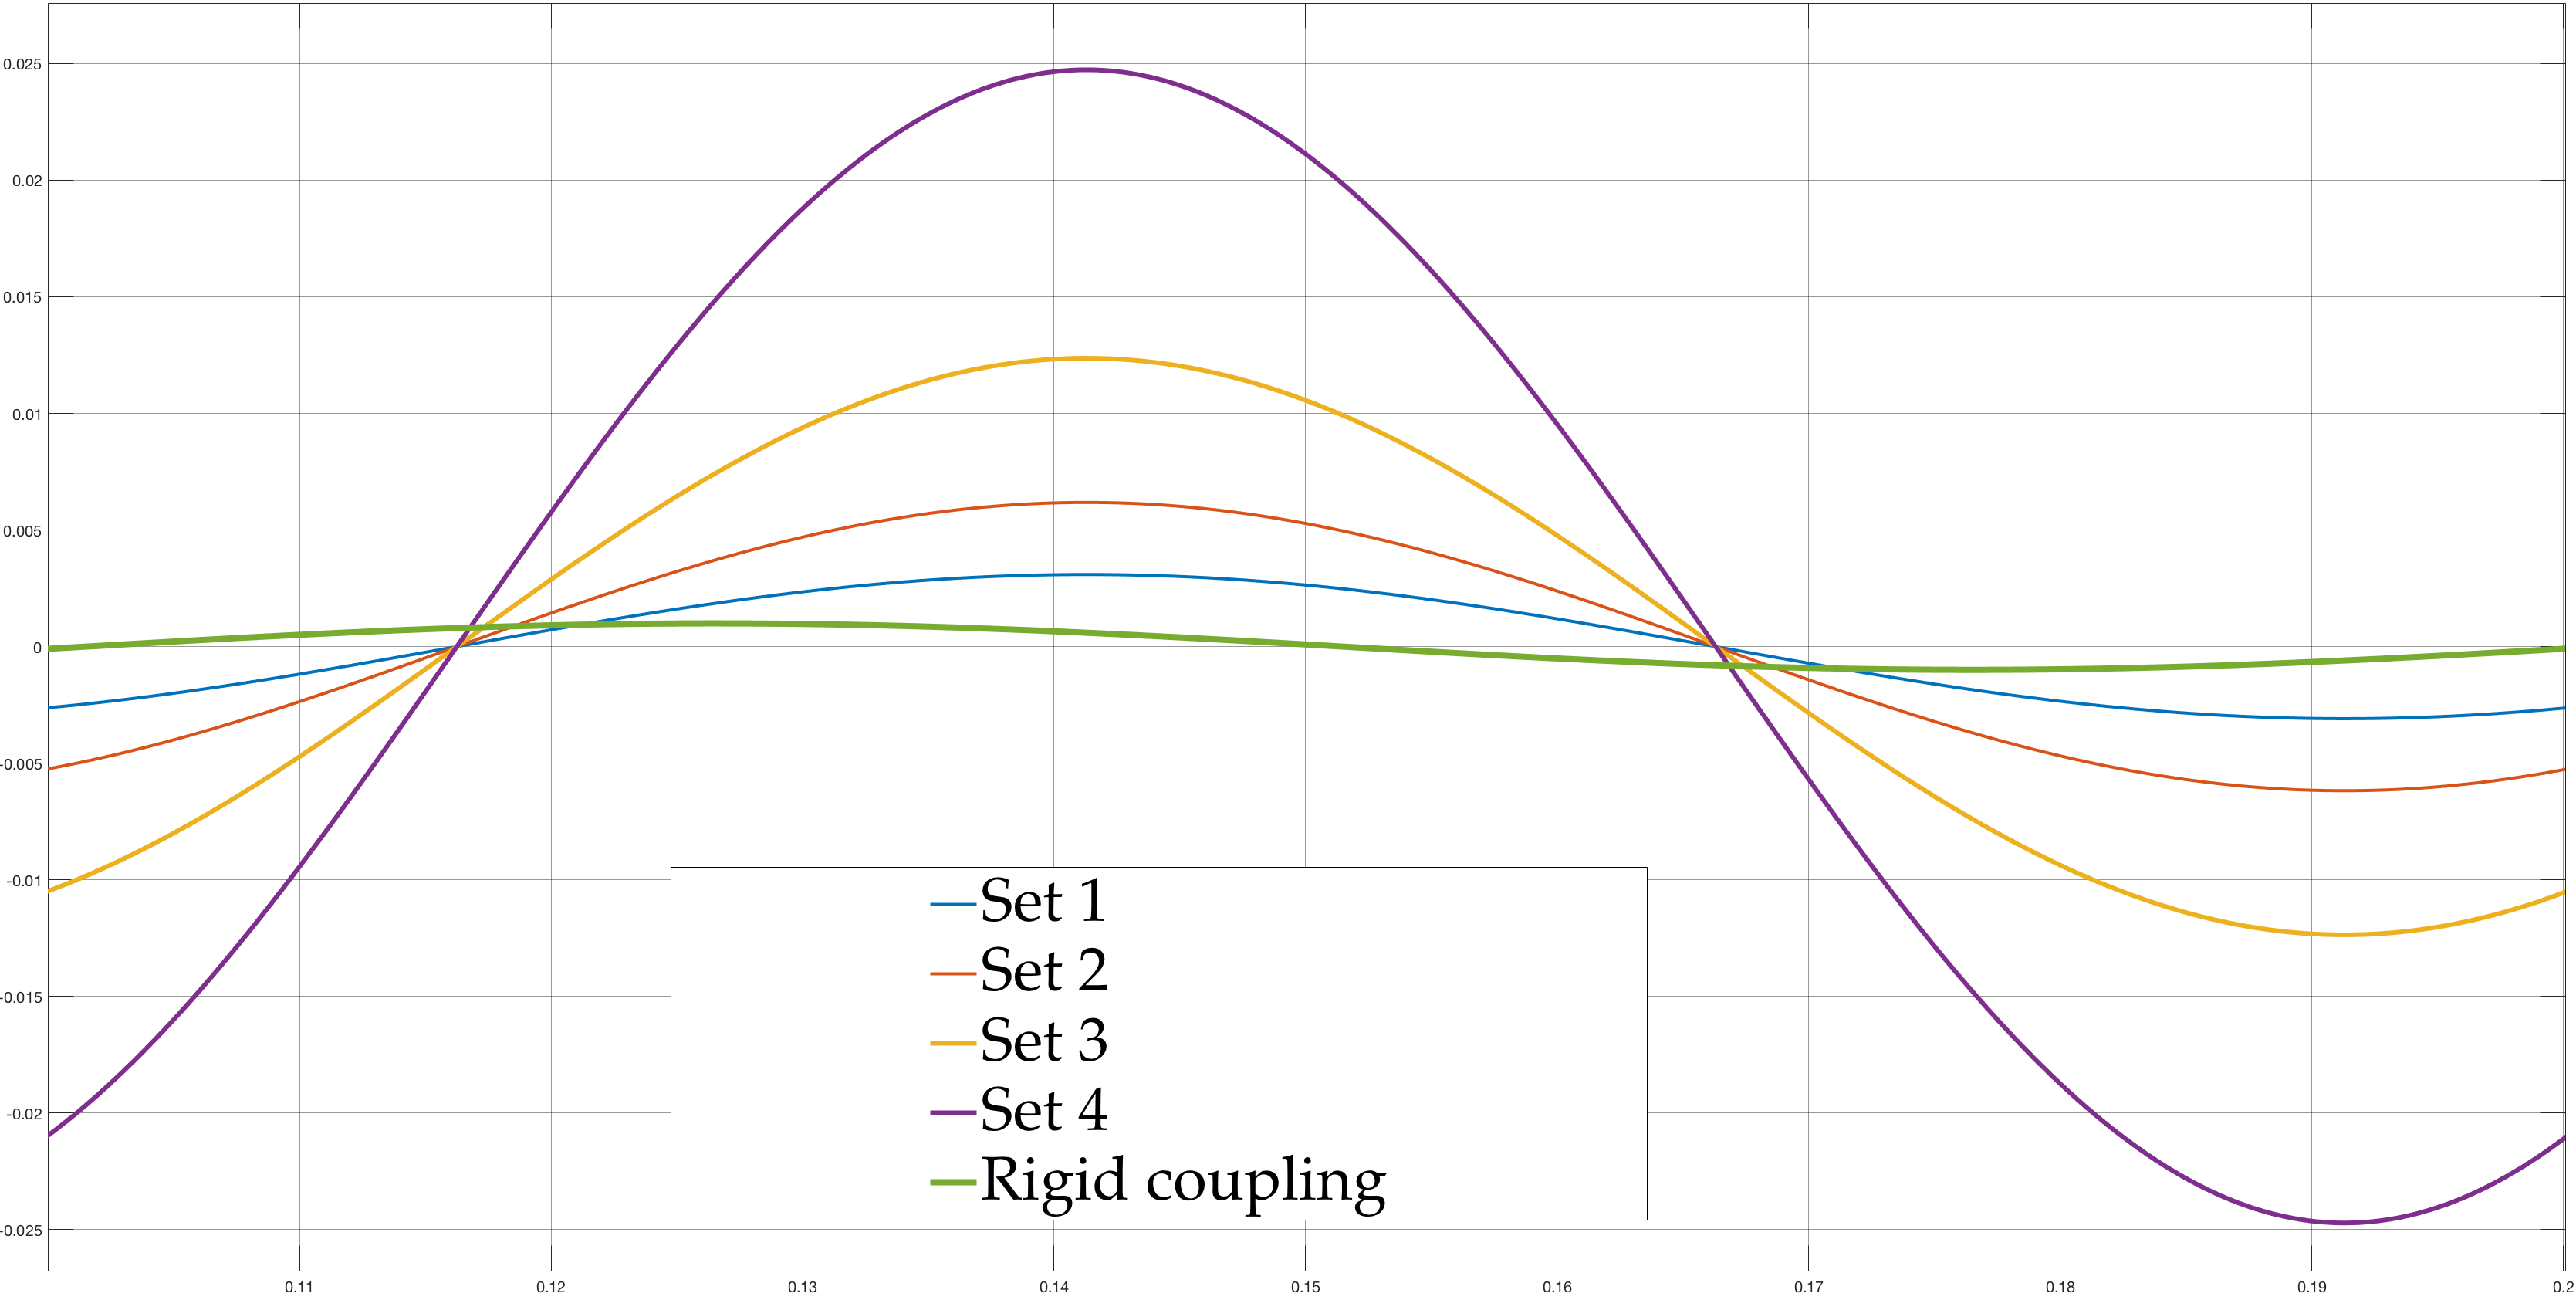
\includegraphics[width=\textwidth, height=0.40\textwidth]{Images/vibr10Htz}
		\caption{10 Hz}
		\label{fig:10Htz}
	\end{subfigure}
\end{figure}
\begin{figure}\ContinuedFloat
	\begin{subfigure}[h!]{1\linewidth}
		\centering
		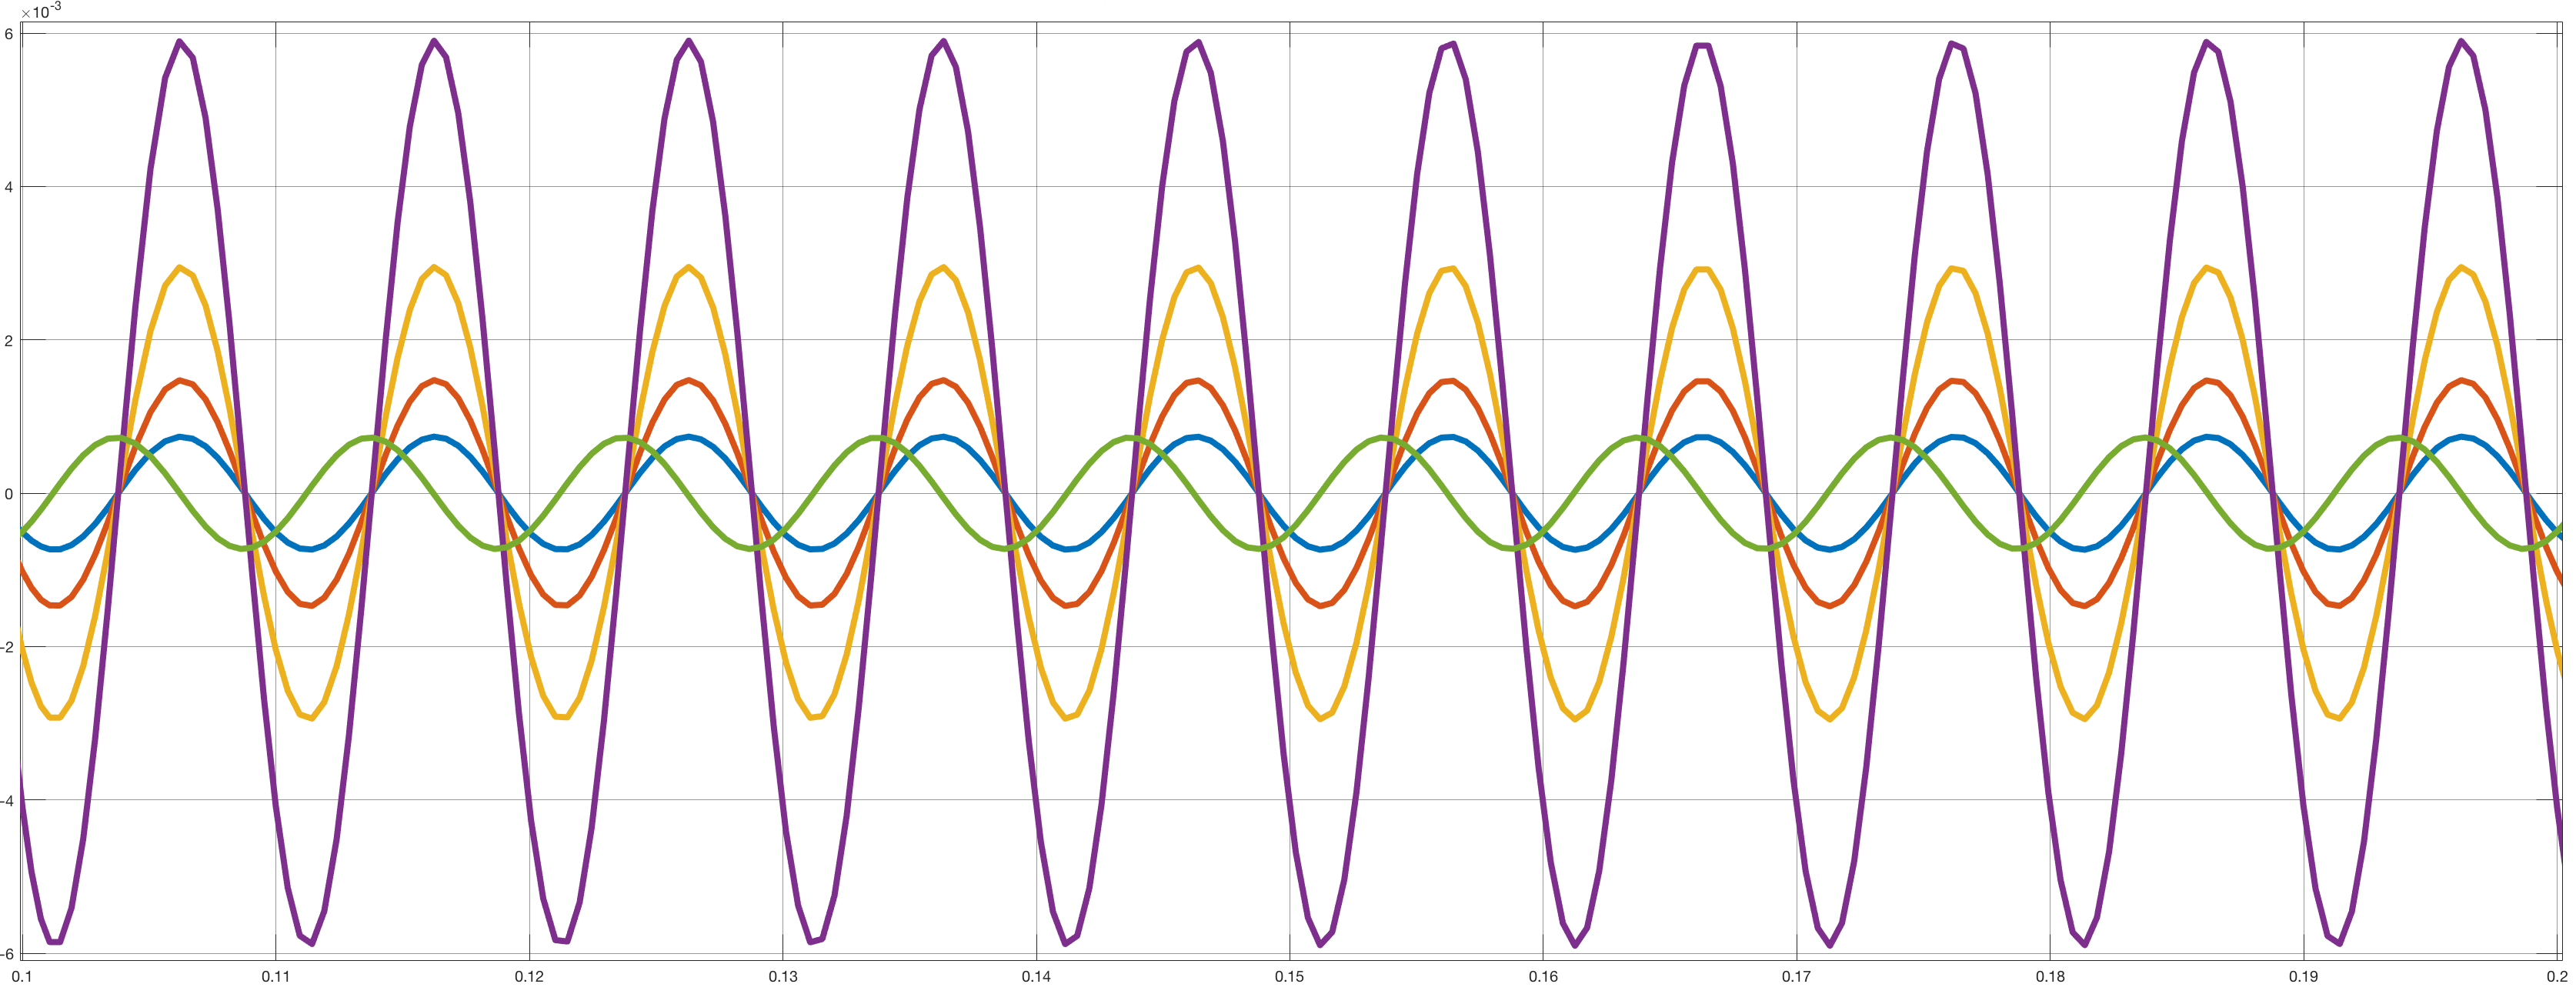
\includegraphics[width=\textwidth, height=0.45\textwidth]{Images/vibr100Htz}
		\caption{100 Hz}
		\label{fig:100Htz}
	\end{subfigure}
\end{figure}
\begin{figure}\ContinuedFloat
	\begin{subfigure}[h!]{1\linewidth}
		\centering.
		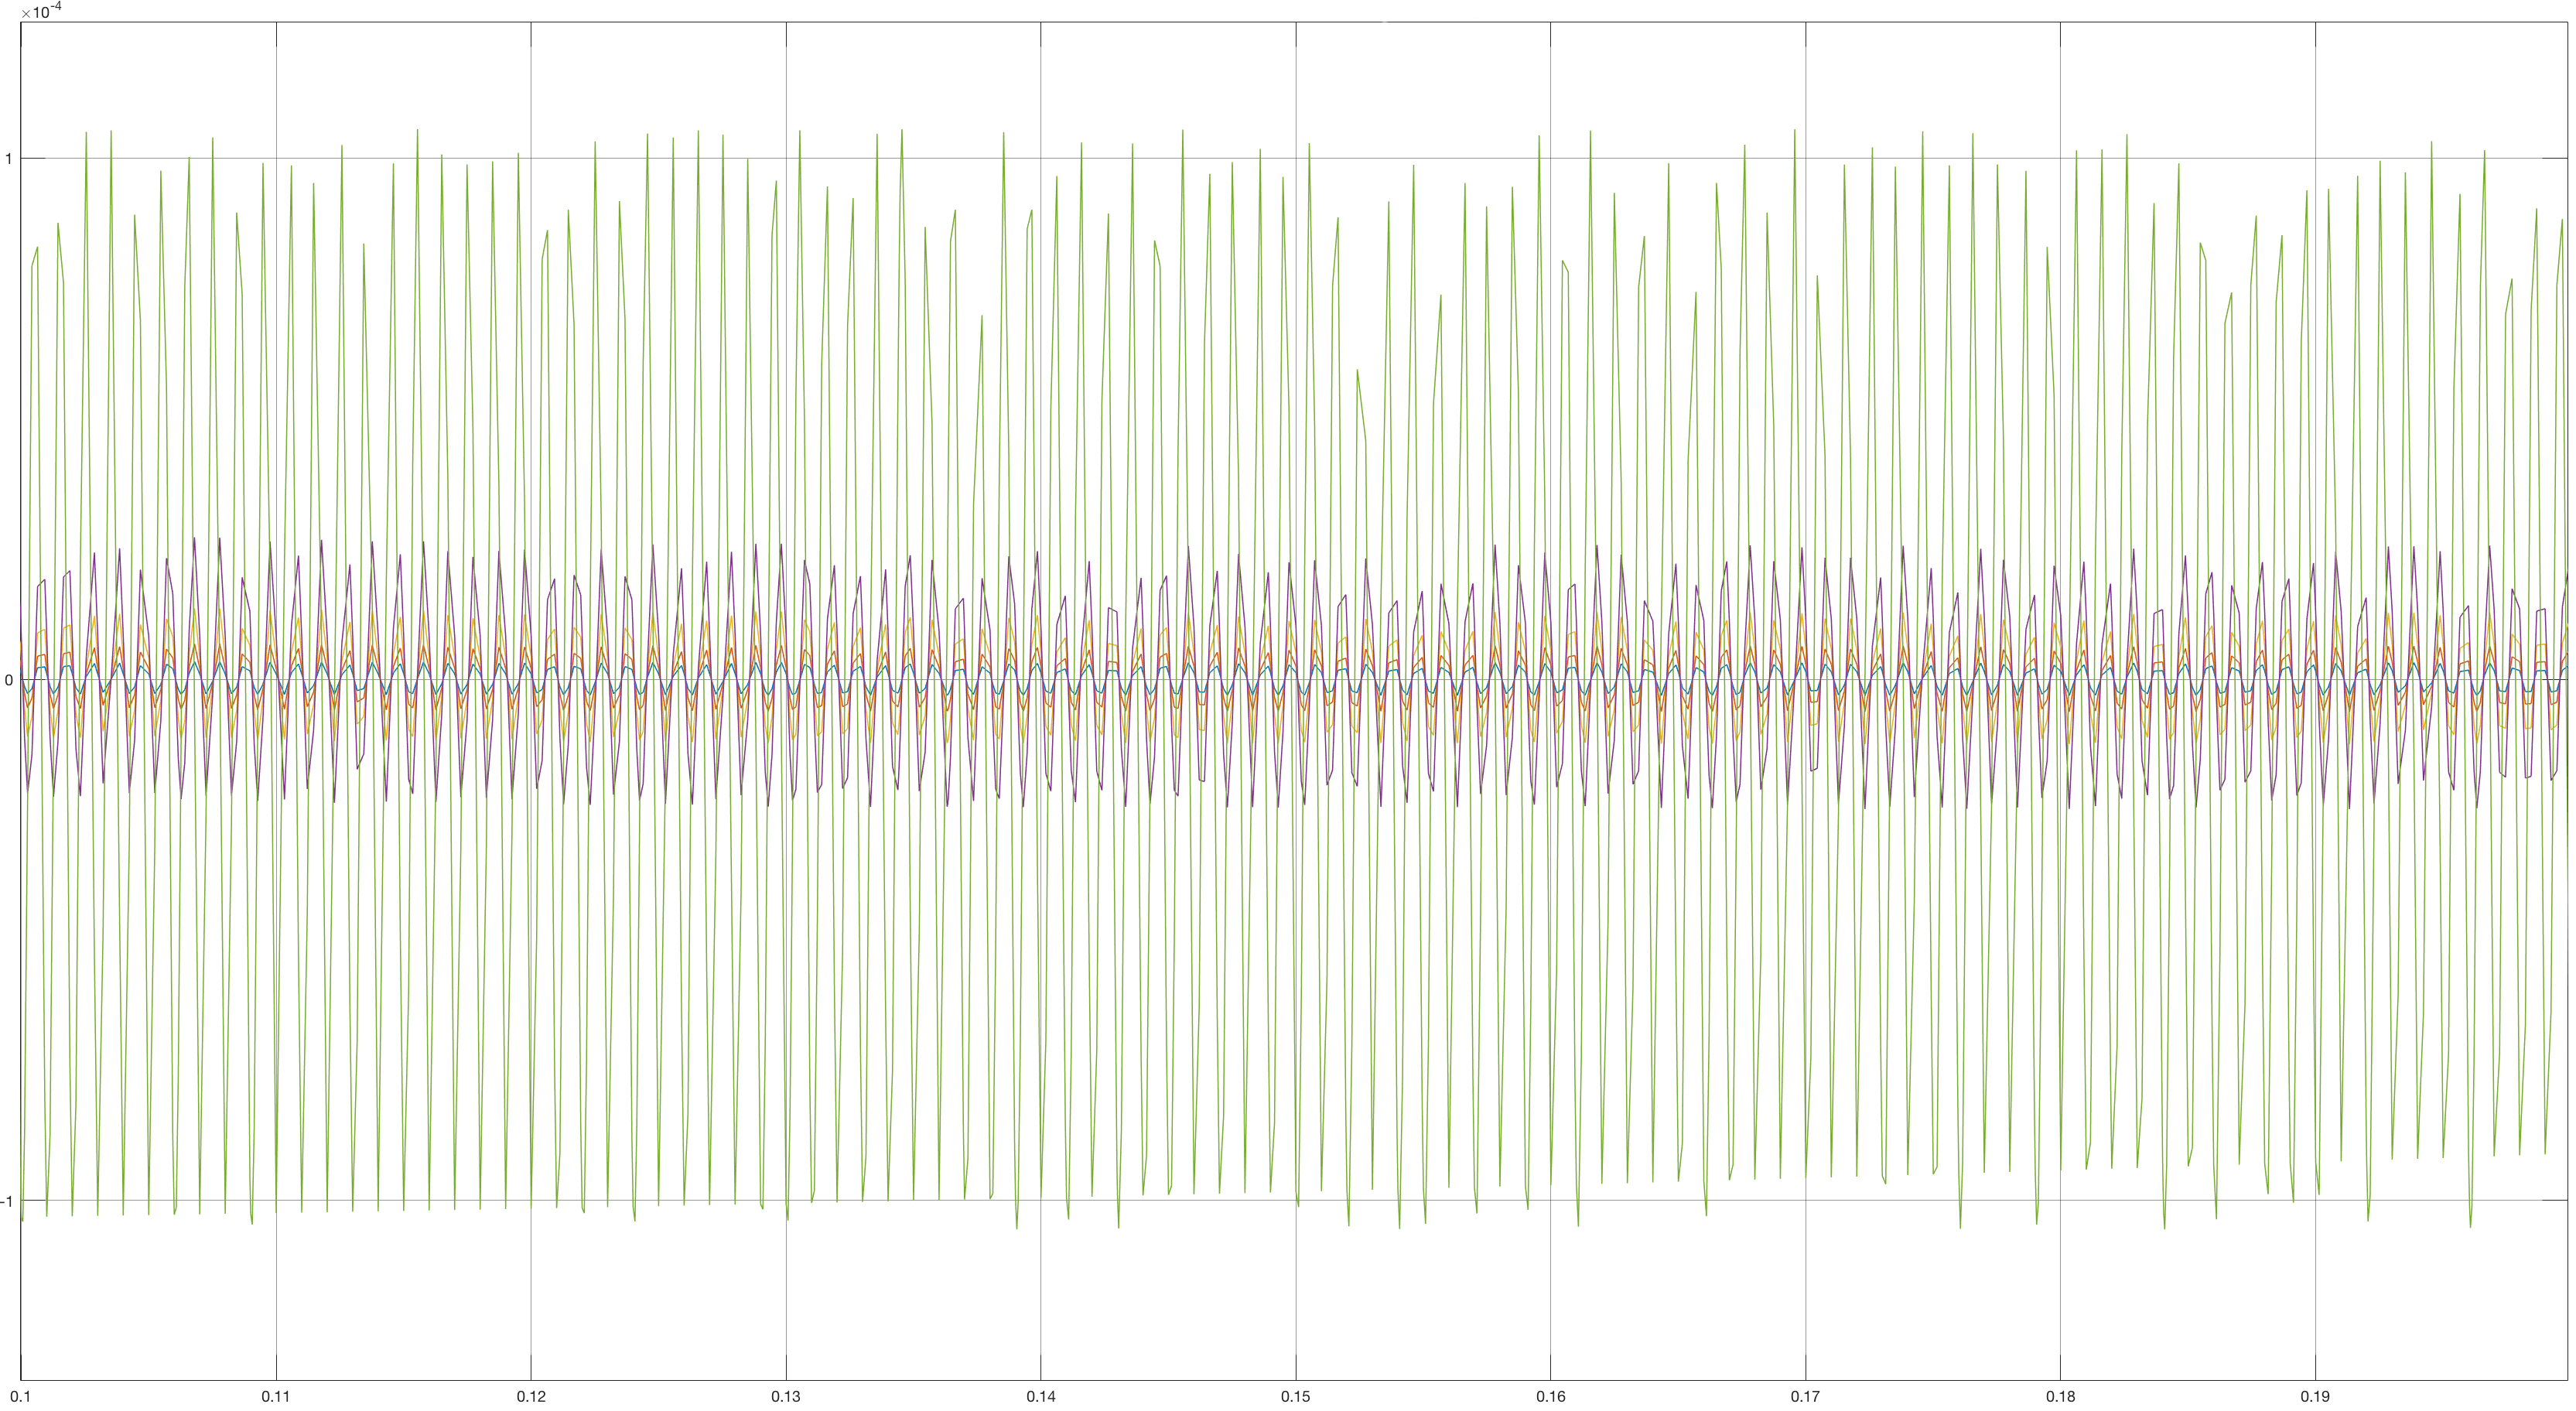
\includegraphics[width=\textwidth, height=0.45\textwidth]{Images/vibr1000Htz}
		\caption{1000 Hz}
		\label{fig:1000Htz}
	\end{subfigure}
\caption{Slave position response to a sinusoidal input with three different frequencies.}
\label{positionResponceFrequencies}
\end{figure}

\subsection{Task execution analysis}

\subsubsection*{Simulation setup}

The operator is modeled as spring-damper system ($ K=200.0 \ \text{N/m} $ and $ B=4.0 \ \text{N}\cdot\text{s}/\text{m} $). The master-slave system has arms of length equal to $ 0.1 \ \text{m} $. 

The environment with which the slave manipulator comes into contact is modeled as:
\begin{itemize}
	\item free motion: the environment has no stiffness but just a small damping $ B_{env}=0.01 \ \text{N}\cdot\text{s}/\text{m} $;
	\item contact motion: the environment has large stiffness $ K_{env} = 4000.0 \ \text{N/m} $ after a chosen value of displacement.
\end{itemize}

The simulation are performed with the \textbf{control set 4} ($ K_v = 20.0 \frac{\text{N m}}{\text{rad}} $, $ B_v = 4.4\cdot 10^{-1} \ \frac{\text{N m}}{\text{rad/s}}$, $ J_v = 3\cdot 10^{-4} \ \text{kg m\textsuperscript{2}}$) and are compared with the \textbf{rigid coupling control} ($K_v = 10^{2} \ \frac{\text{N m}}{\text{rad}} $, $B_v = 1.5\cdot 10^{-1} \ \frac{\text{N m}}{\text{rad/s}}$, $J_v =  0 \ \text{kg m\textsuperscript{2}} $).

\subsubsection{Free motion with high frequency input}

At first, we present an execution in free motion. The slave manages to mirror the master which is moved according to a $ 0.11 \ \text{Hz} $ sinusoidal trajectory. Applying both \textsl{rigid coupling control} (fig.\ref{fig:freeRigTot50HR}) and \textsl{virtual compliance control} (fig.\ref{fig:freeSetTot50HR}) there is almost no task error.
% with almost no task error (without considering the error due to noise disturbances).

The noise of the system is modeled as a mixture of white noise and sinusoidal oscillations both at frequency of $50 \ \text{Hz}$ on the slave side.

\begin{figure}[H]
	\begin{subfigure}{1\linewidth}
		\centering
		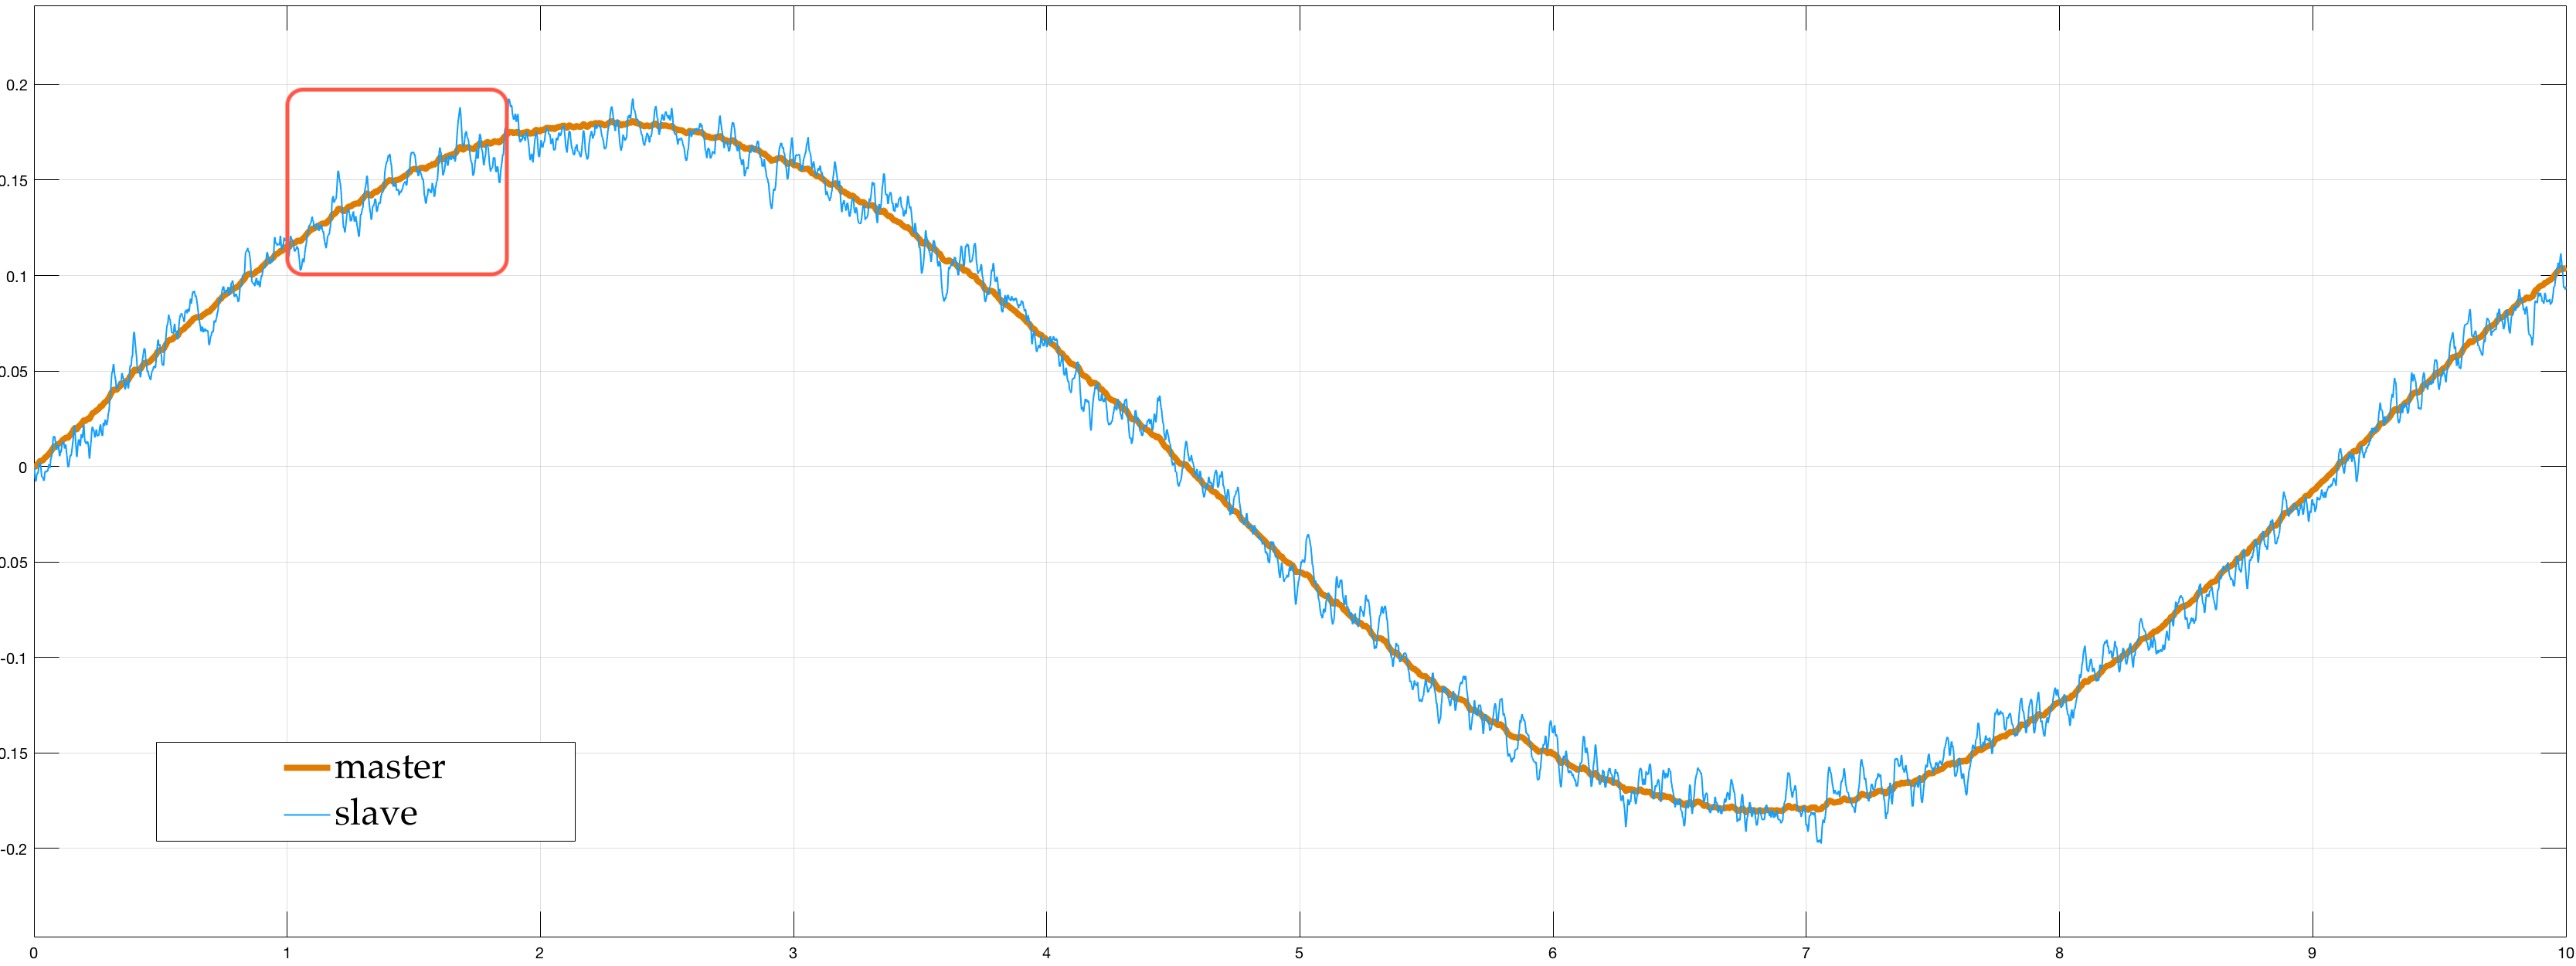
\includegraphics[width=\textwidth, height=0.48\textwidth]{Images/set20freeTot50HtznoiseRect}
		\caption{Positions of the master-slave system in free motion - virtual compliance control.}
		\label{fig:freeSetTot50HR}
	\end{subfigure}	
\end{figure}
\begin{figure}[H]\ContinuedFloat
	\begin{subfigure}{1\linewidth}
		\centering
		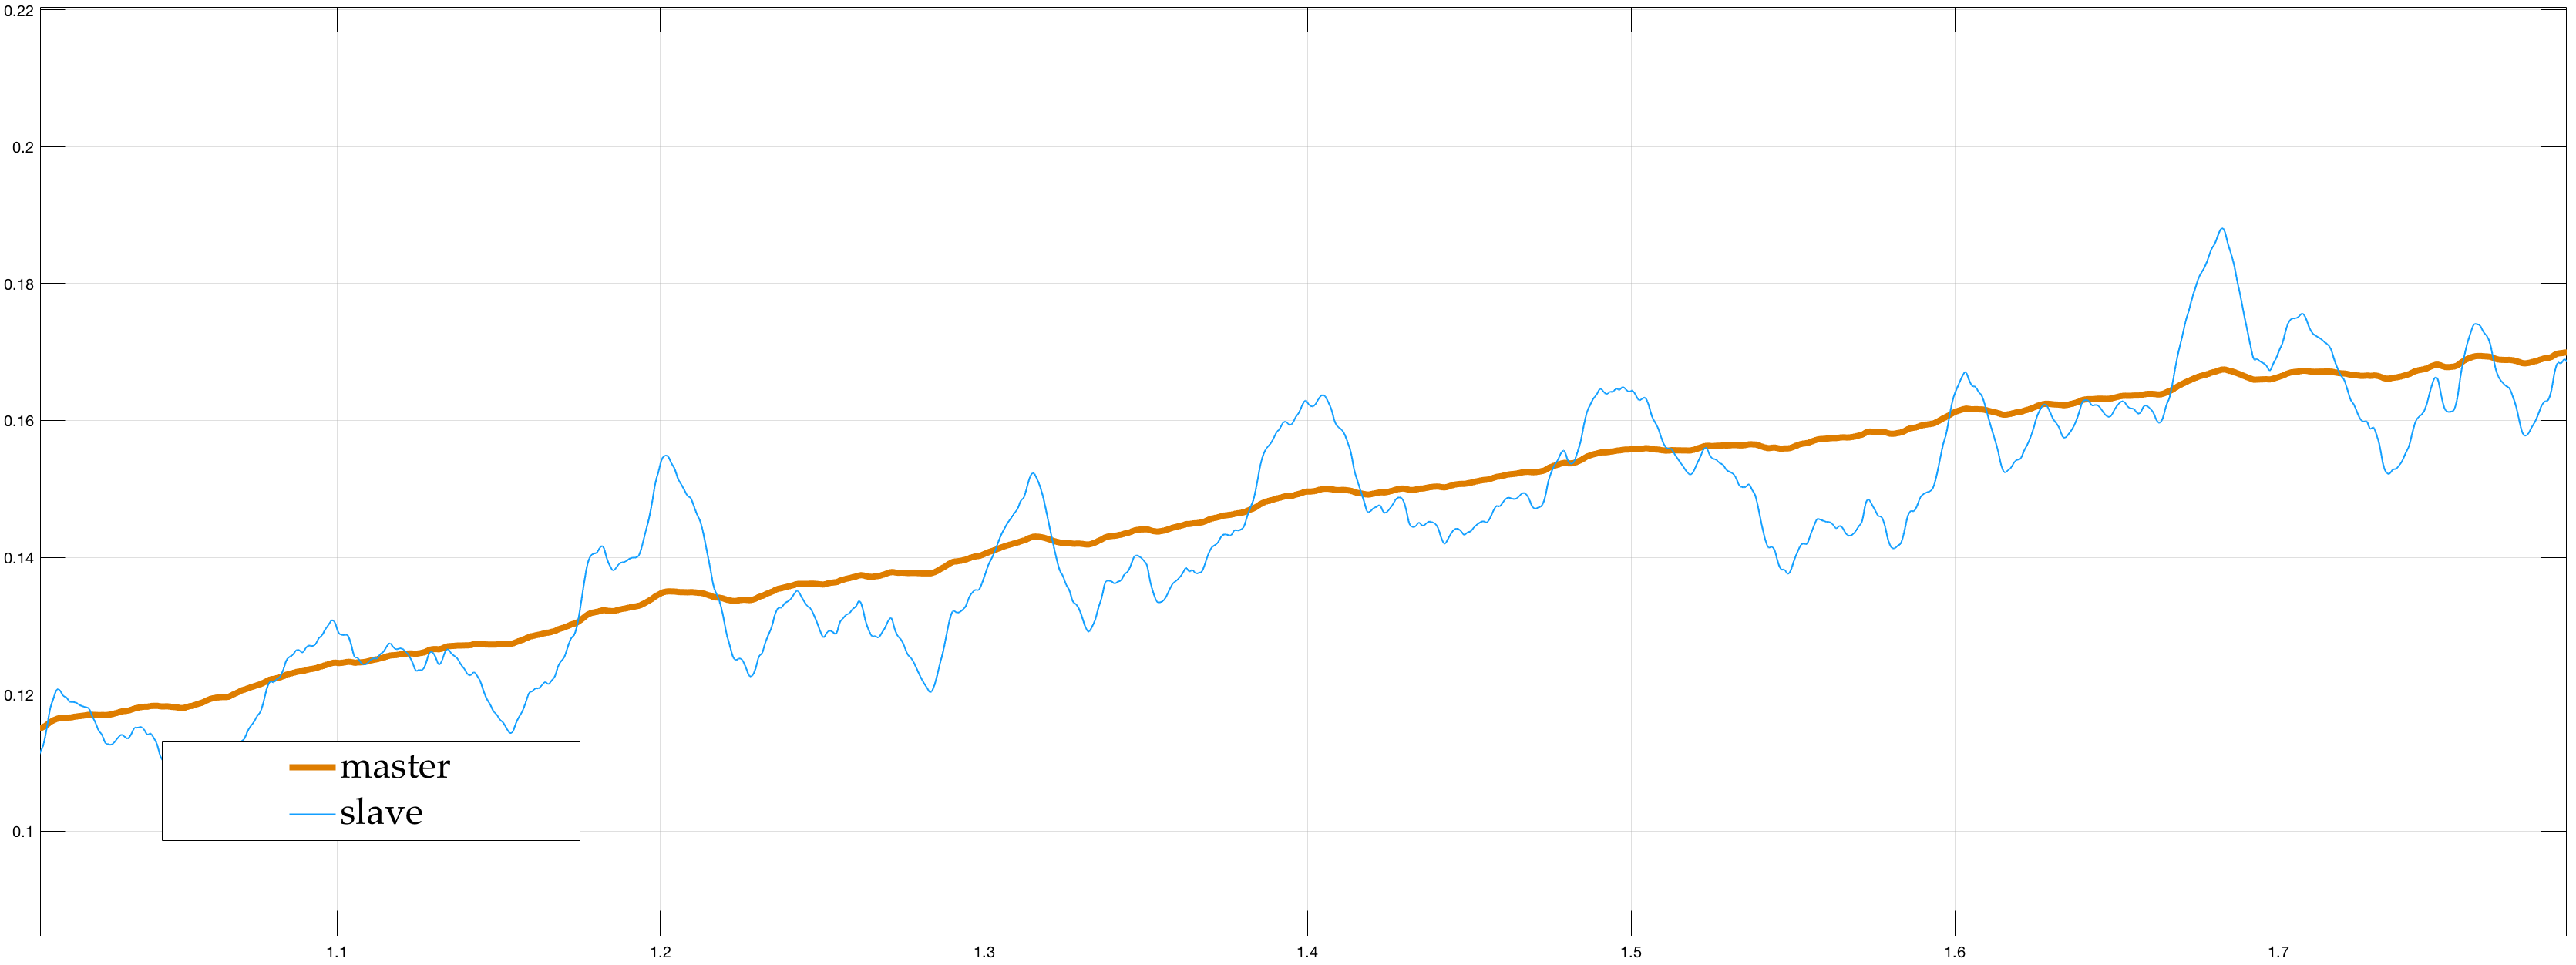
\includegraphics[width=\textwidth, height=0.48\textwidth]{Images/set20freePart50Htznoise}
		\caption{Detail describing the highlighted area in fig.\ref{fig:freeSetTot50HR}}
		\label{fig:freeSetPar50HR}
	\end{subfigure}	
	\caption{\textbf{High} frequency disturbances response - virtual compliance control.}
\end{figure}

\begin{figure}[H]
	\begin{subfigure}{1\linewidth}
		\centering
		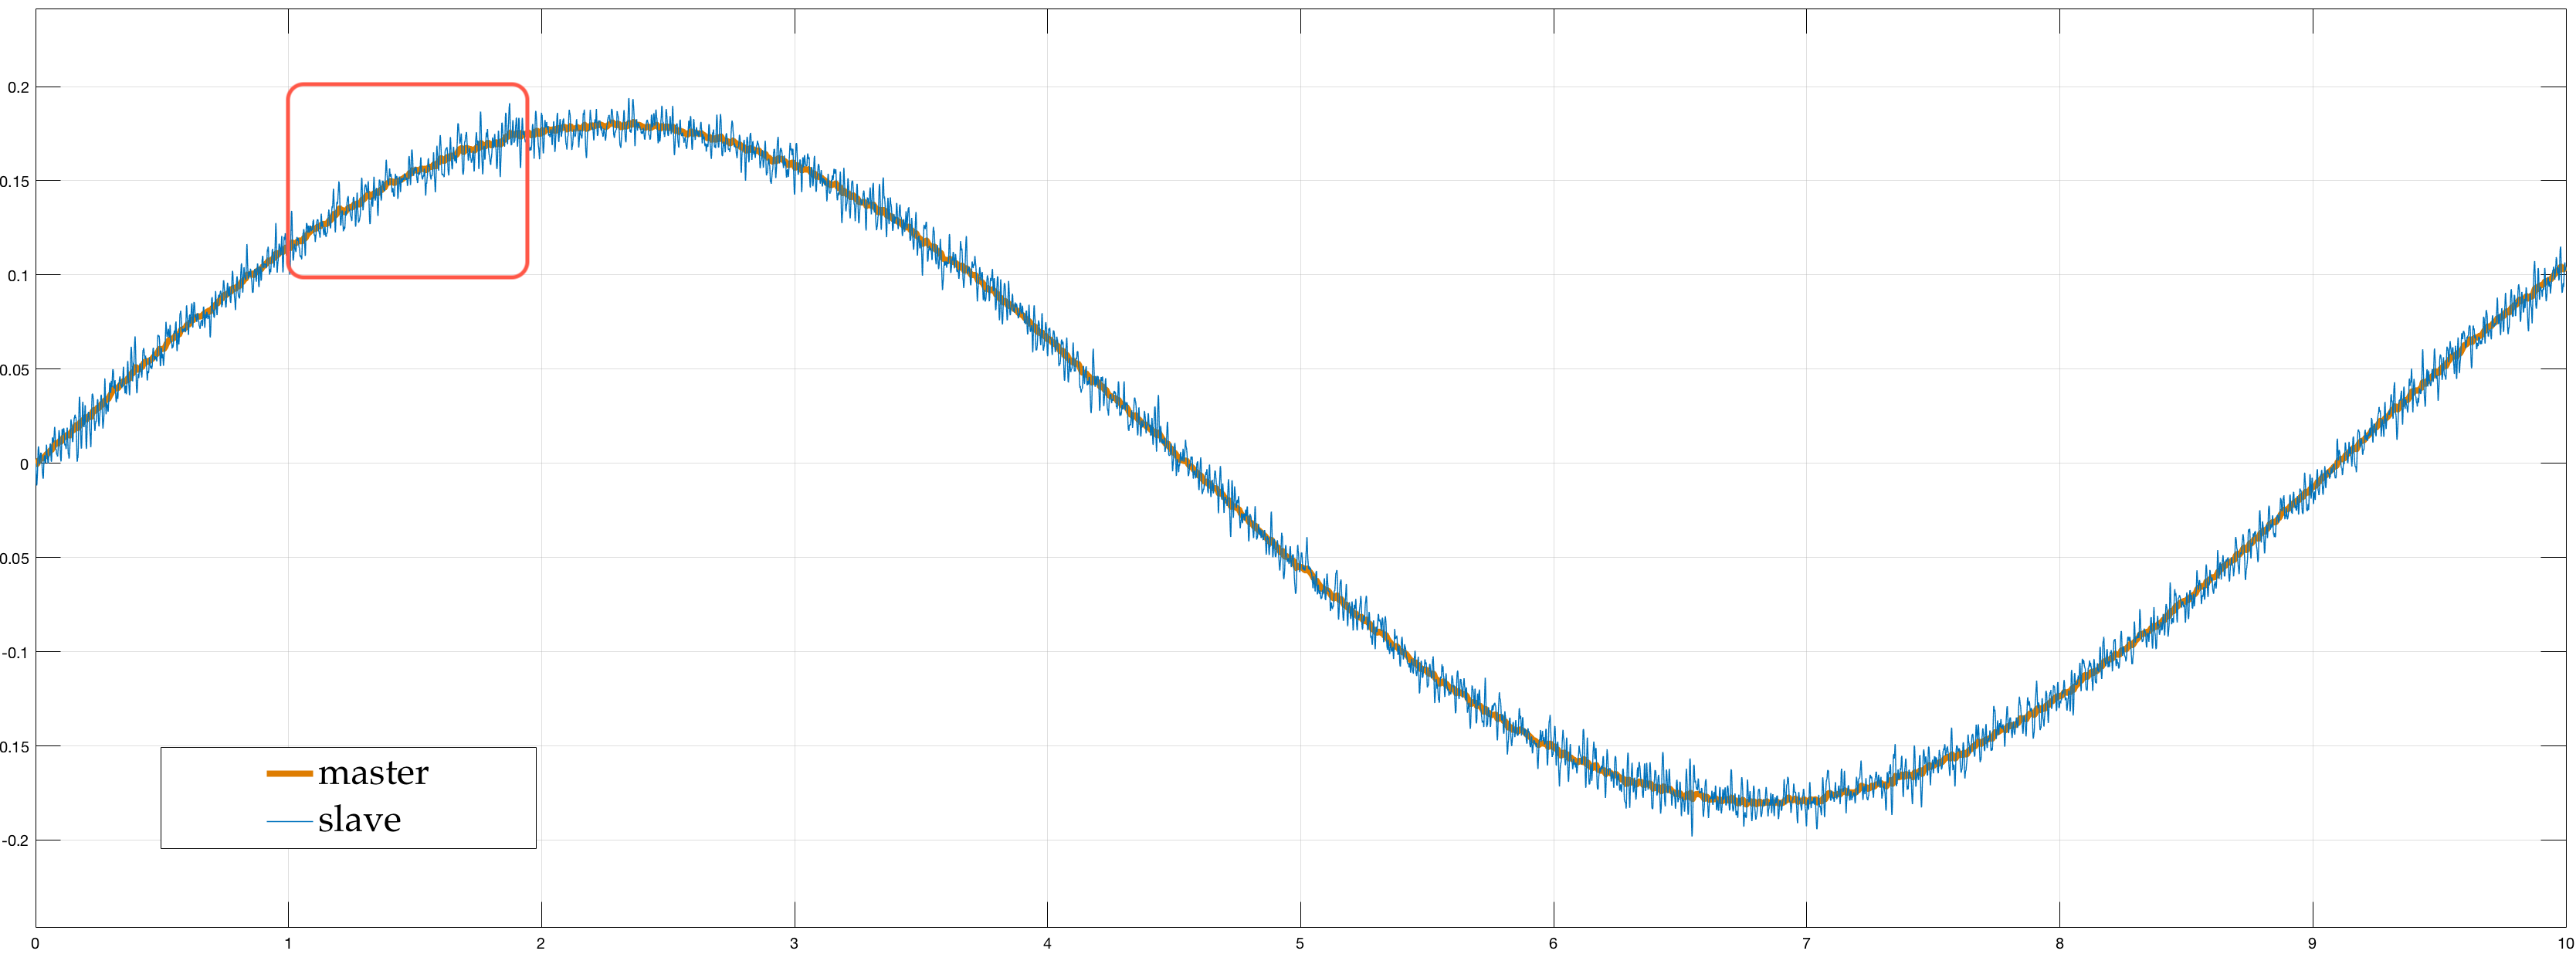
\includegraphics[width=\textwidth, height=0.48\textwidth]{Images/rCoupFreeTot50htznoiseRect}
		\caption{Positions of the master-slave system in free motion - rigid coupling control.}
		\label{fig:freeRigTot50HR}
	\end{subfigure}
\end{figure}
\begin{figure}[H]\ContinuedFloat
	\begin{subfigure}{1\linewidth}
		\centering
		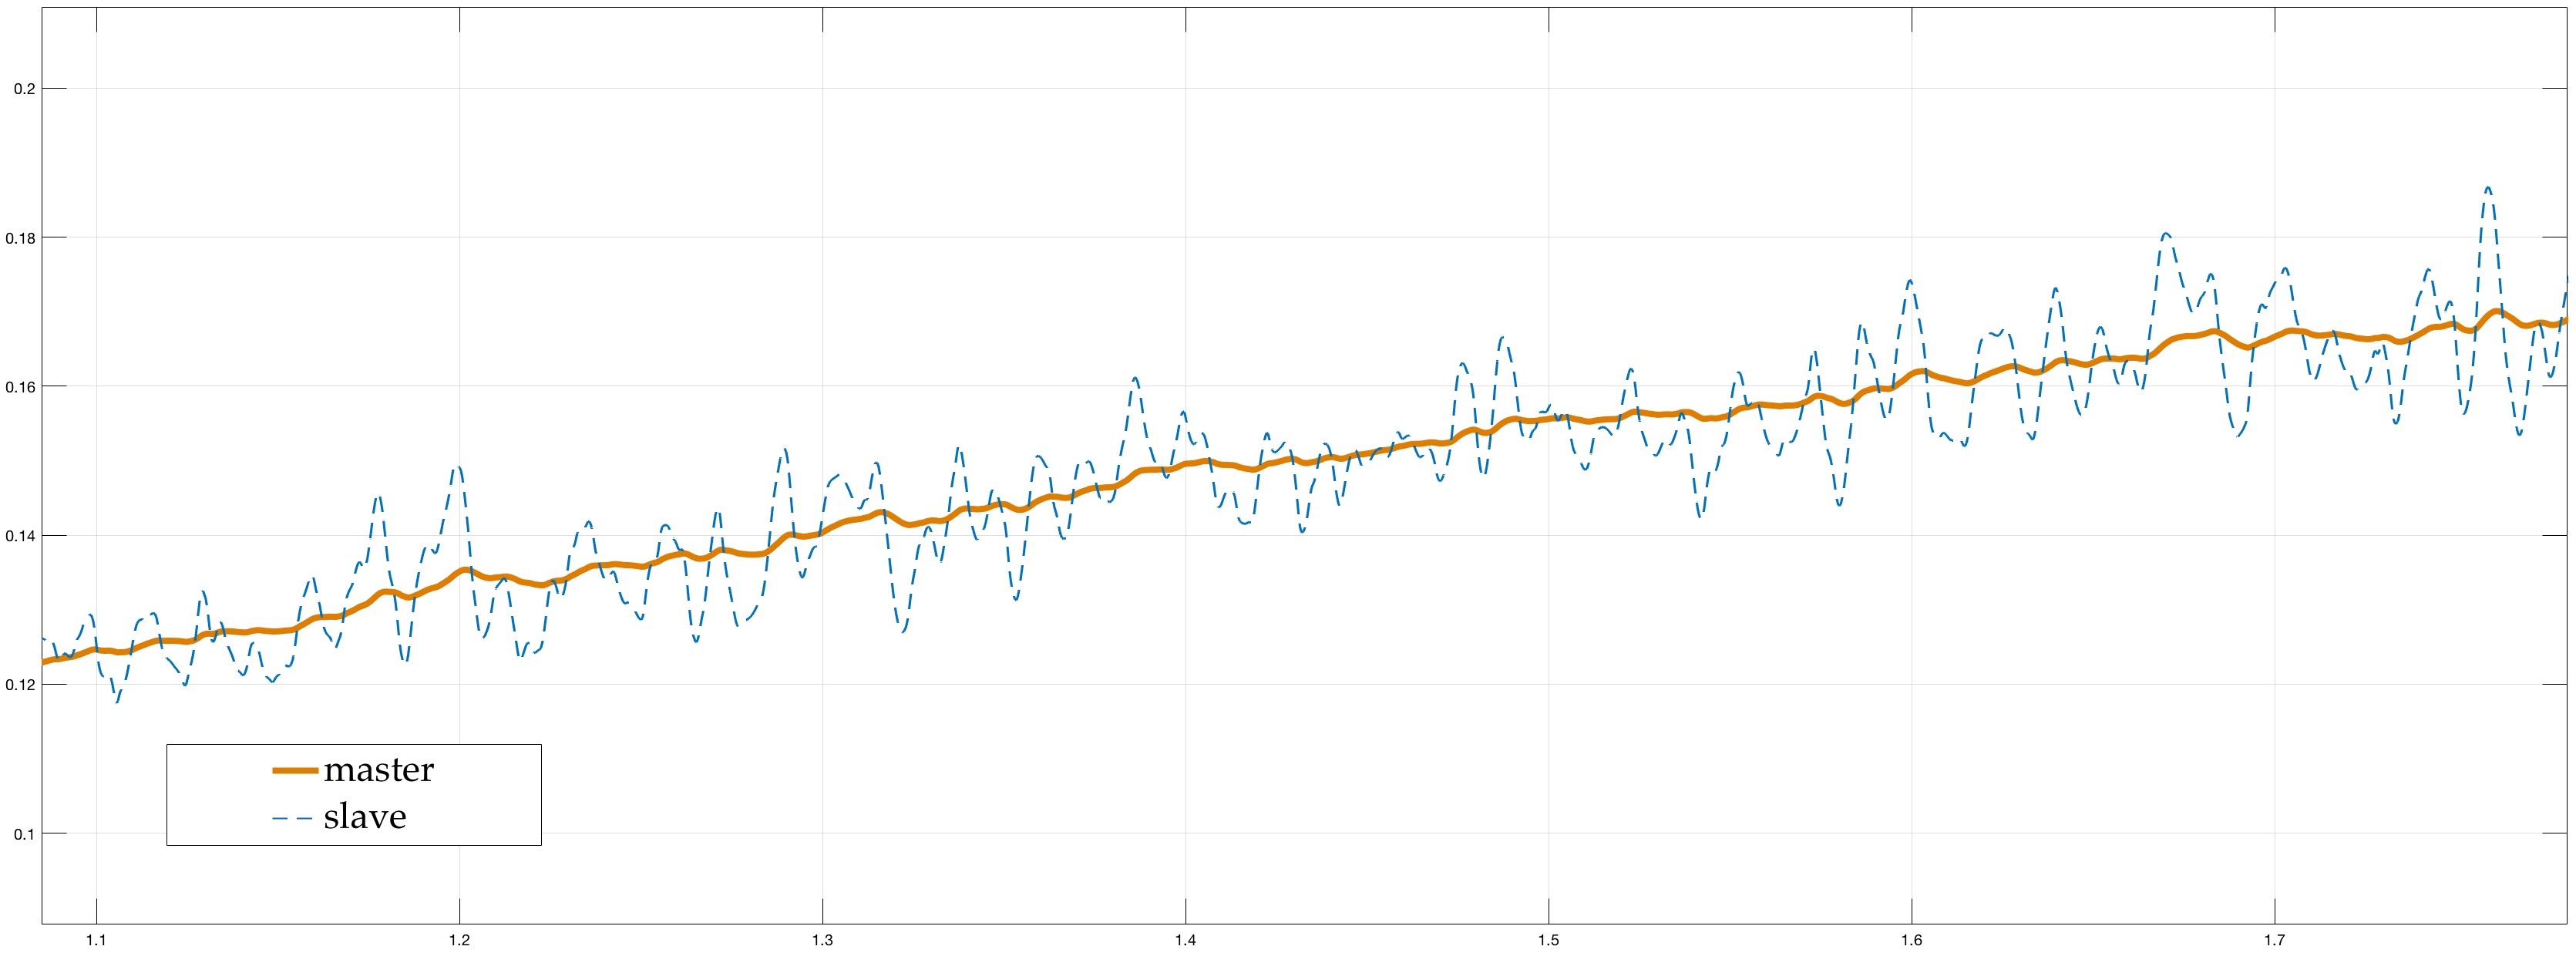
\includegraphics[width=\textwidth, height=0.48\textwidth]{Images/rCoupFree50htznoise}
		\caption{Detail describing the highlighted area in fig.\ref{fig:freeRigTot50HR}.}
		\label{fig:freeRigPar50HR}
	\end{subfigure}	
  \caption{\textbf{High} frequency disturbances response - rigid coupling control.}
\end{figure}

%This kind of disturbance should be damped, and in fact, using \textsl{virtual compliance} (fig.\ref{fig:freeRigPar50HR}) the profile of the angle is smoother than in \textsl{rigid coupling} (fig.\ref{fig:freeRigPar50HR}).

A comparison between the fig.\ref{fig:freeRigPar50HR} and the fig.\ref{fig:freeSetPar50HR} shows how is the slave response under the two different type of controllers: the response is slower using the virtual compliance control respect to the rigid coupling control. By consequence, the operator "feels" less disturbances. 

\subsubsection{Free motion with low frequency input}

Comparatively, two other simulations have been performed under the same
conditions of the previous ones. Here the input frequency is lowered to $20.0 \ \text{Hz}$.

Usually, one wants this type of inputs to be detectable, and hence, they should be preserved. 
%This kind of input are usually a similar to the input of the control
%actuators, so it should be preserved, namely it shouldn't be affected by the
%proposed filtering.

\begin{figure}[H]
	\begin{subfigure}{1\linewidth}
		\centering
		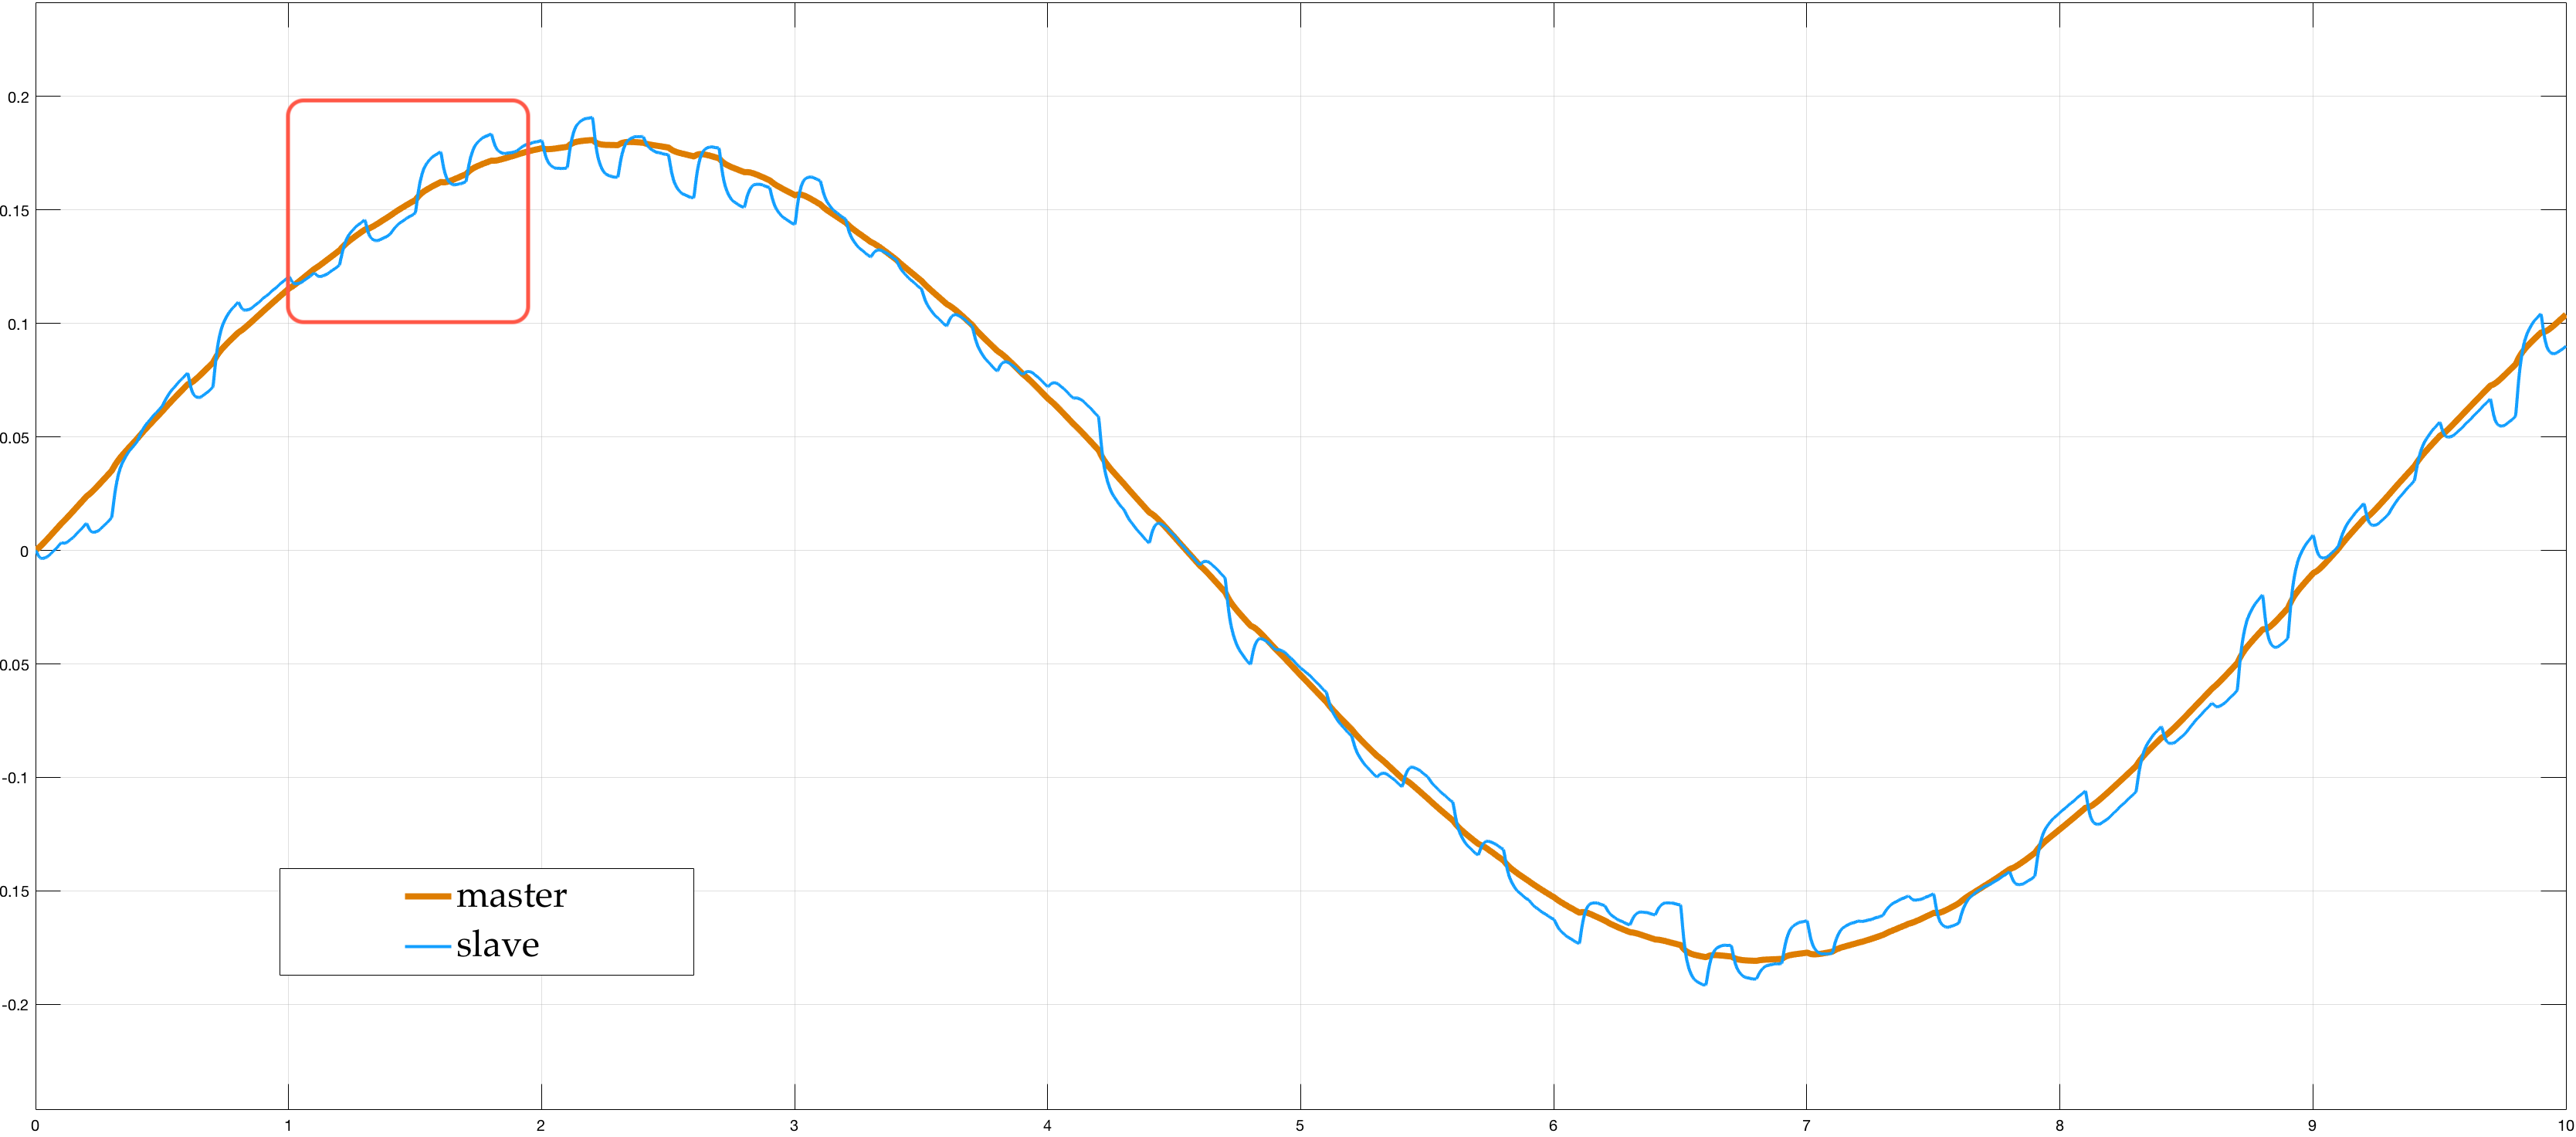
\includegraphics[width=\textwidth, height=0.48\textwidth]{Images/freeSet20Tot20HtznoiseRect}
		\caption{Positions of the master-slave system in free motion - virtual compliance control.}
		\label{fig:freeSetTot20HR}
	\end{subfigure}
\end{figure}
\begin{figure}[H]\ContinuedFloat
	\begin{subfigure}{1\linewidth}
		\centering
		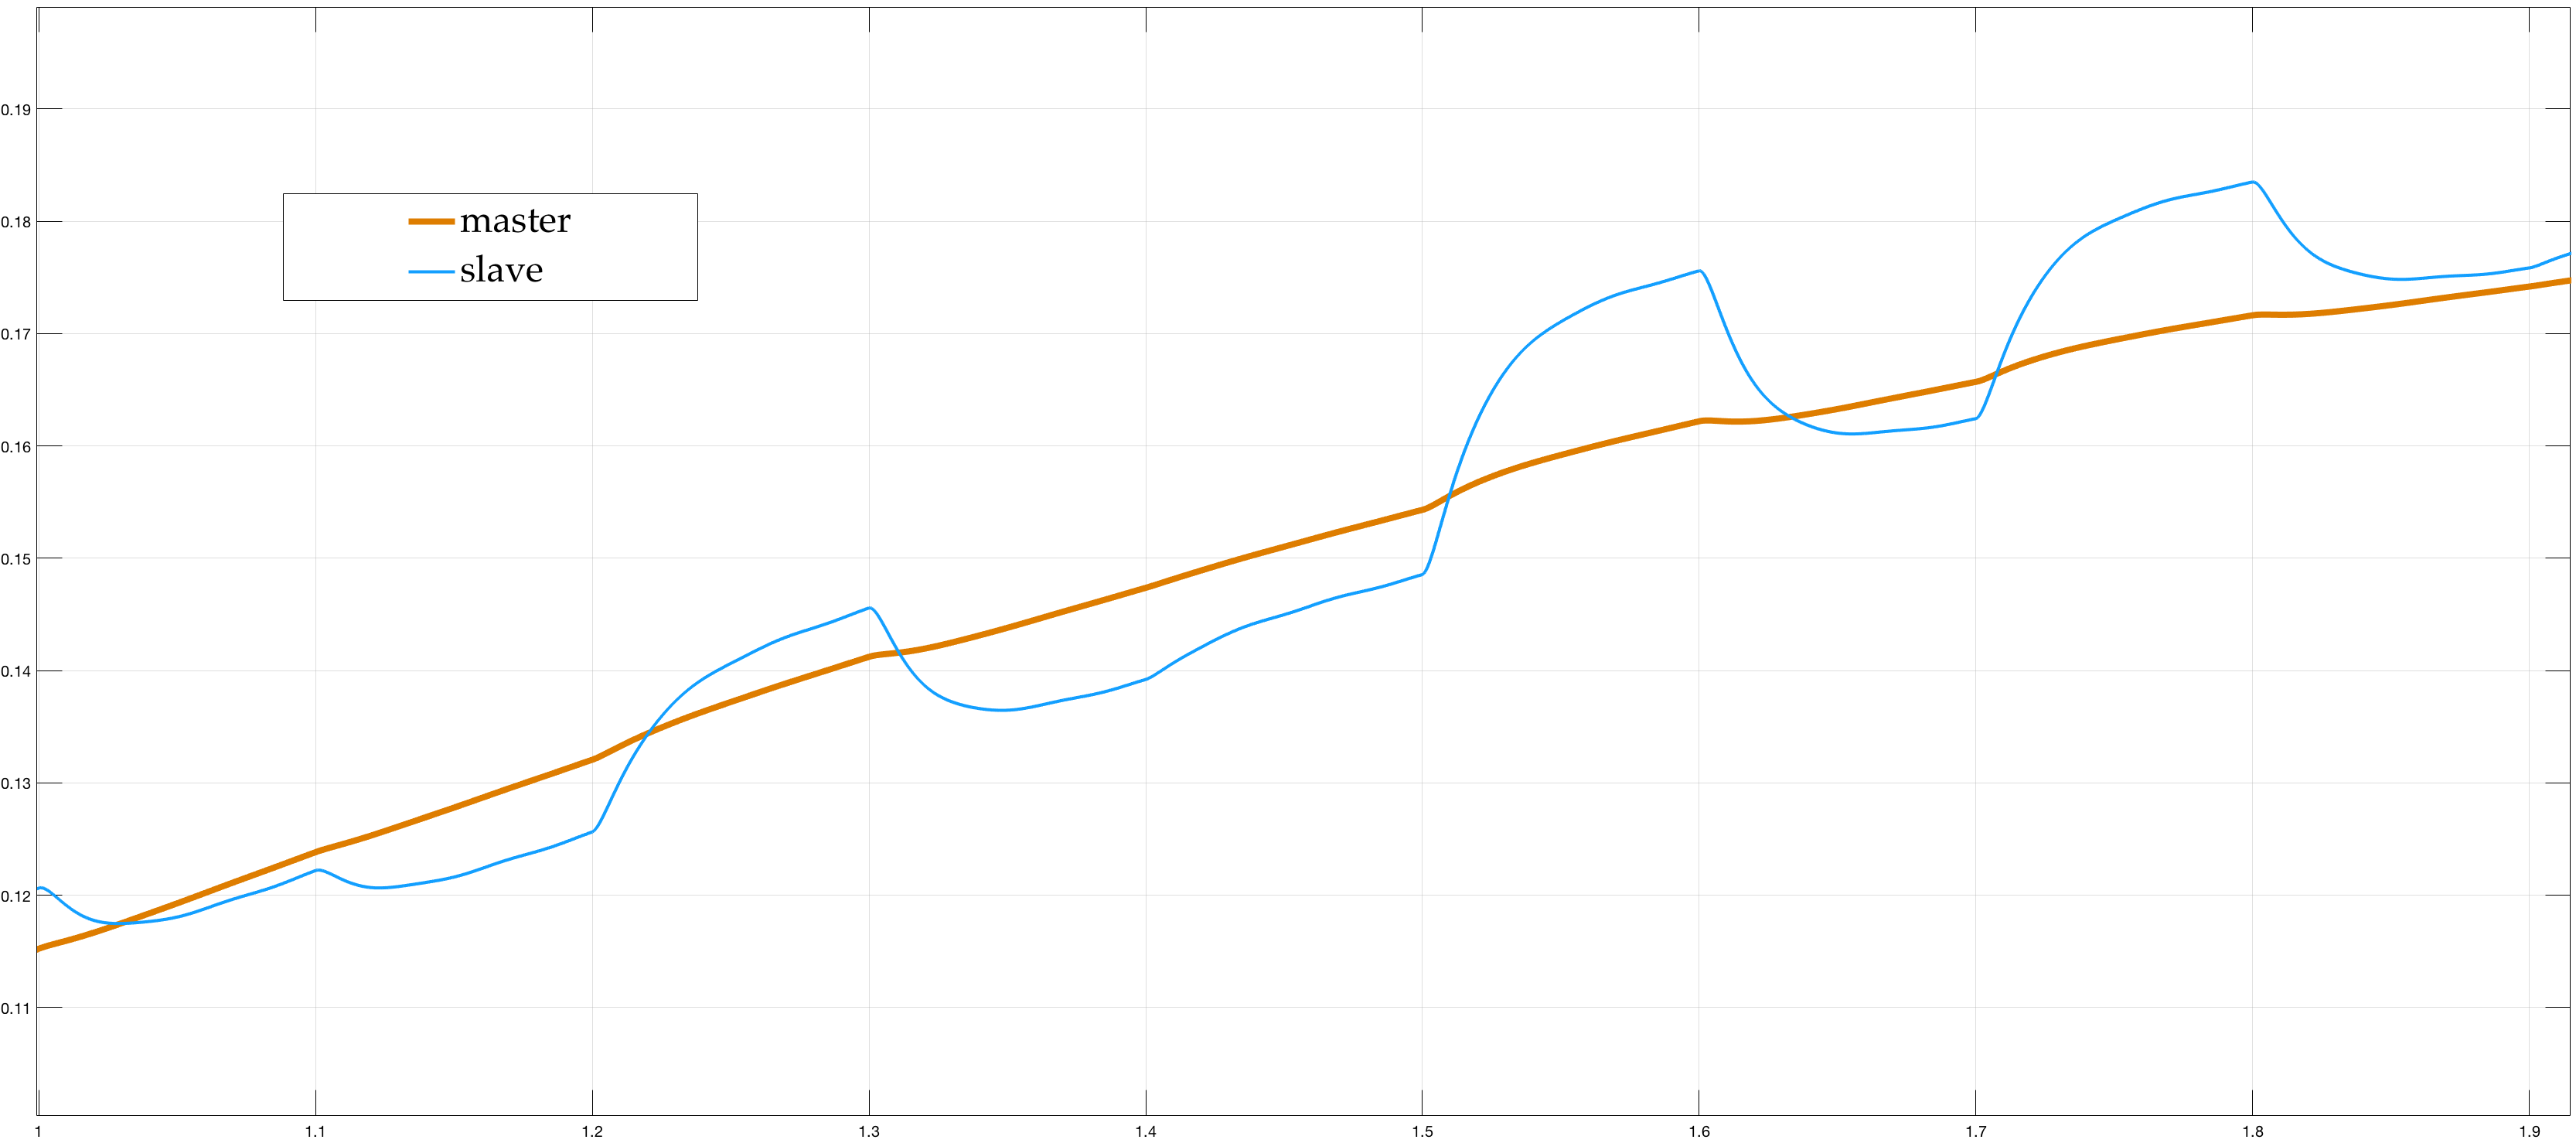
\includegraphics[width=\textwidth, height=0.48\textwidth]{Images/freeSet20Part20Htznoise}
		\caption{Detail describing the highlighted area in fig.\ref{fig:freeSetTot20HR}}
		\label{fig:freeSetPar20HR}
	\end{subfigure}	
	\caption{\textbf{Low} frequency disturbances response - virtual compliance control.}
\end{figure}

\begin{figure}[H]
	\begin{subfigure}{1\linewidth}
		\centering
		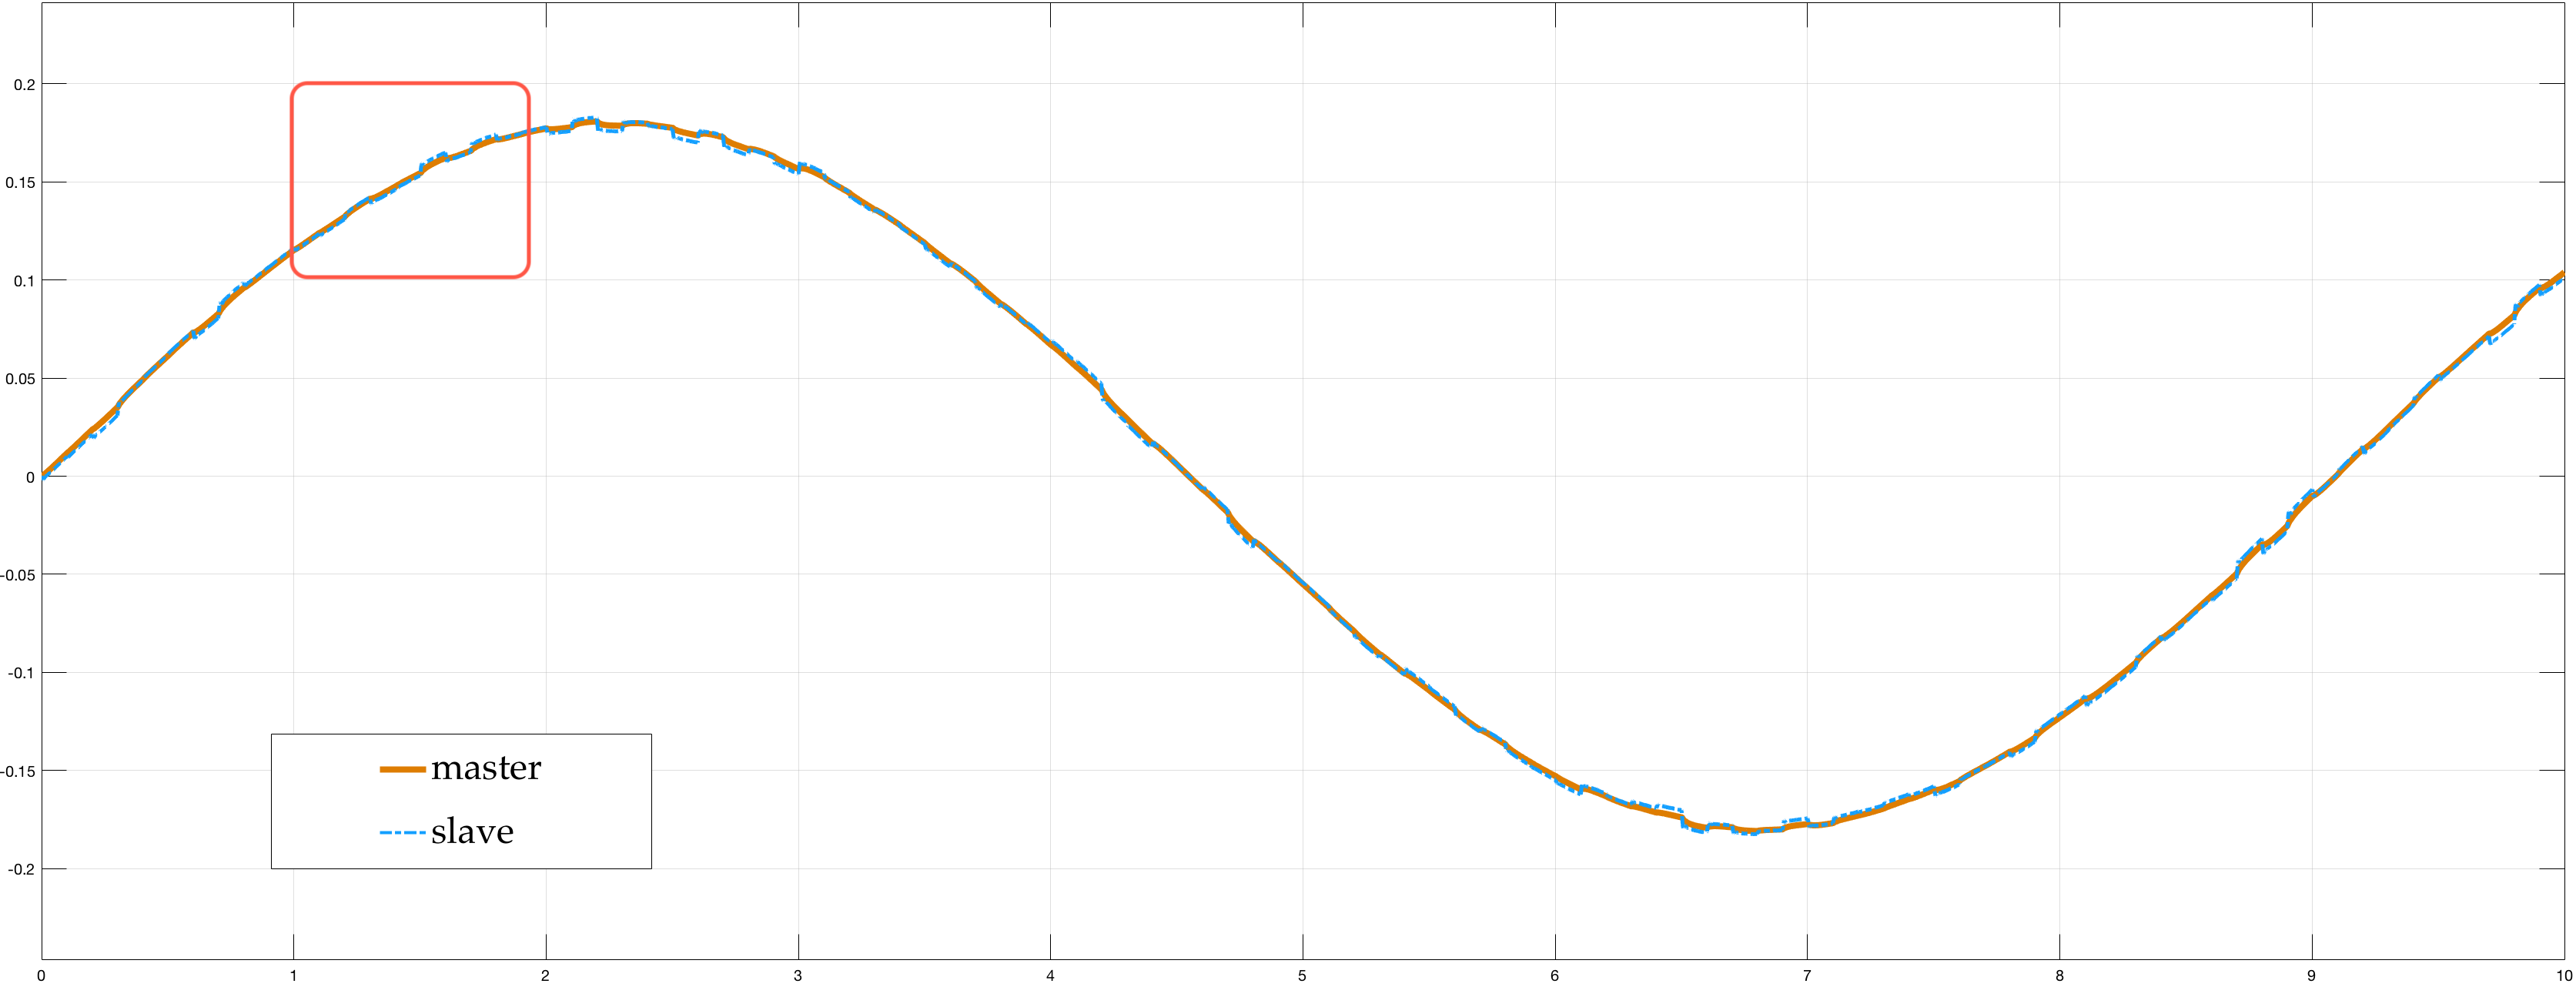
\includegraphics[width=\textwidth, height=0.48\textwidth]{Images/freerigidTot20HtznoiseRect}
		\caption{Positions of the master-slave system in free motion - rigid coupling control.}
		\label{fig:freeRigTot20HR}
	\end{subfigure}	
\end{figure}
\begin{figure}[H]\ContinuedFloat
	\begin{subfigure}{1\linewidth}
		\centering
		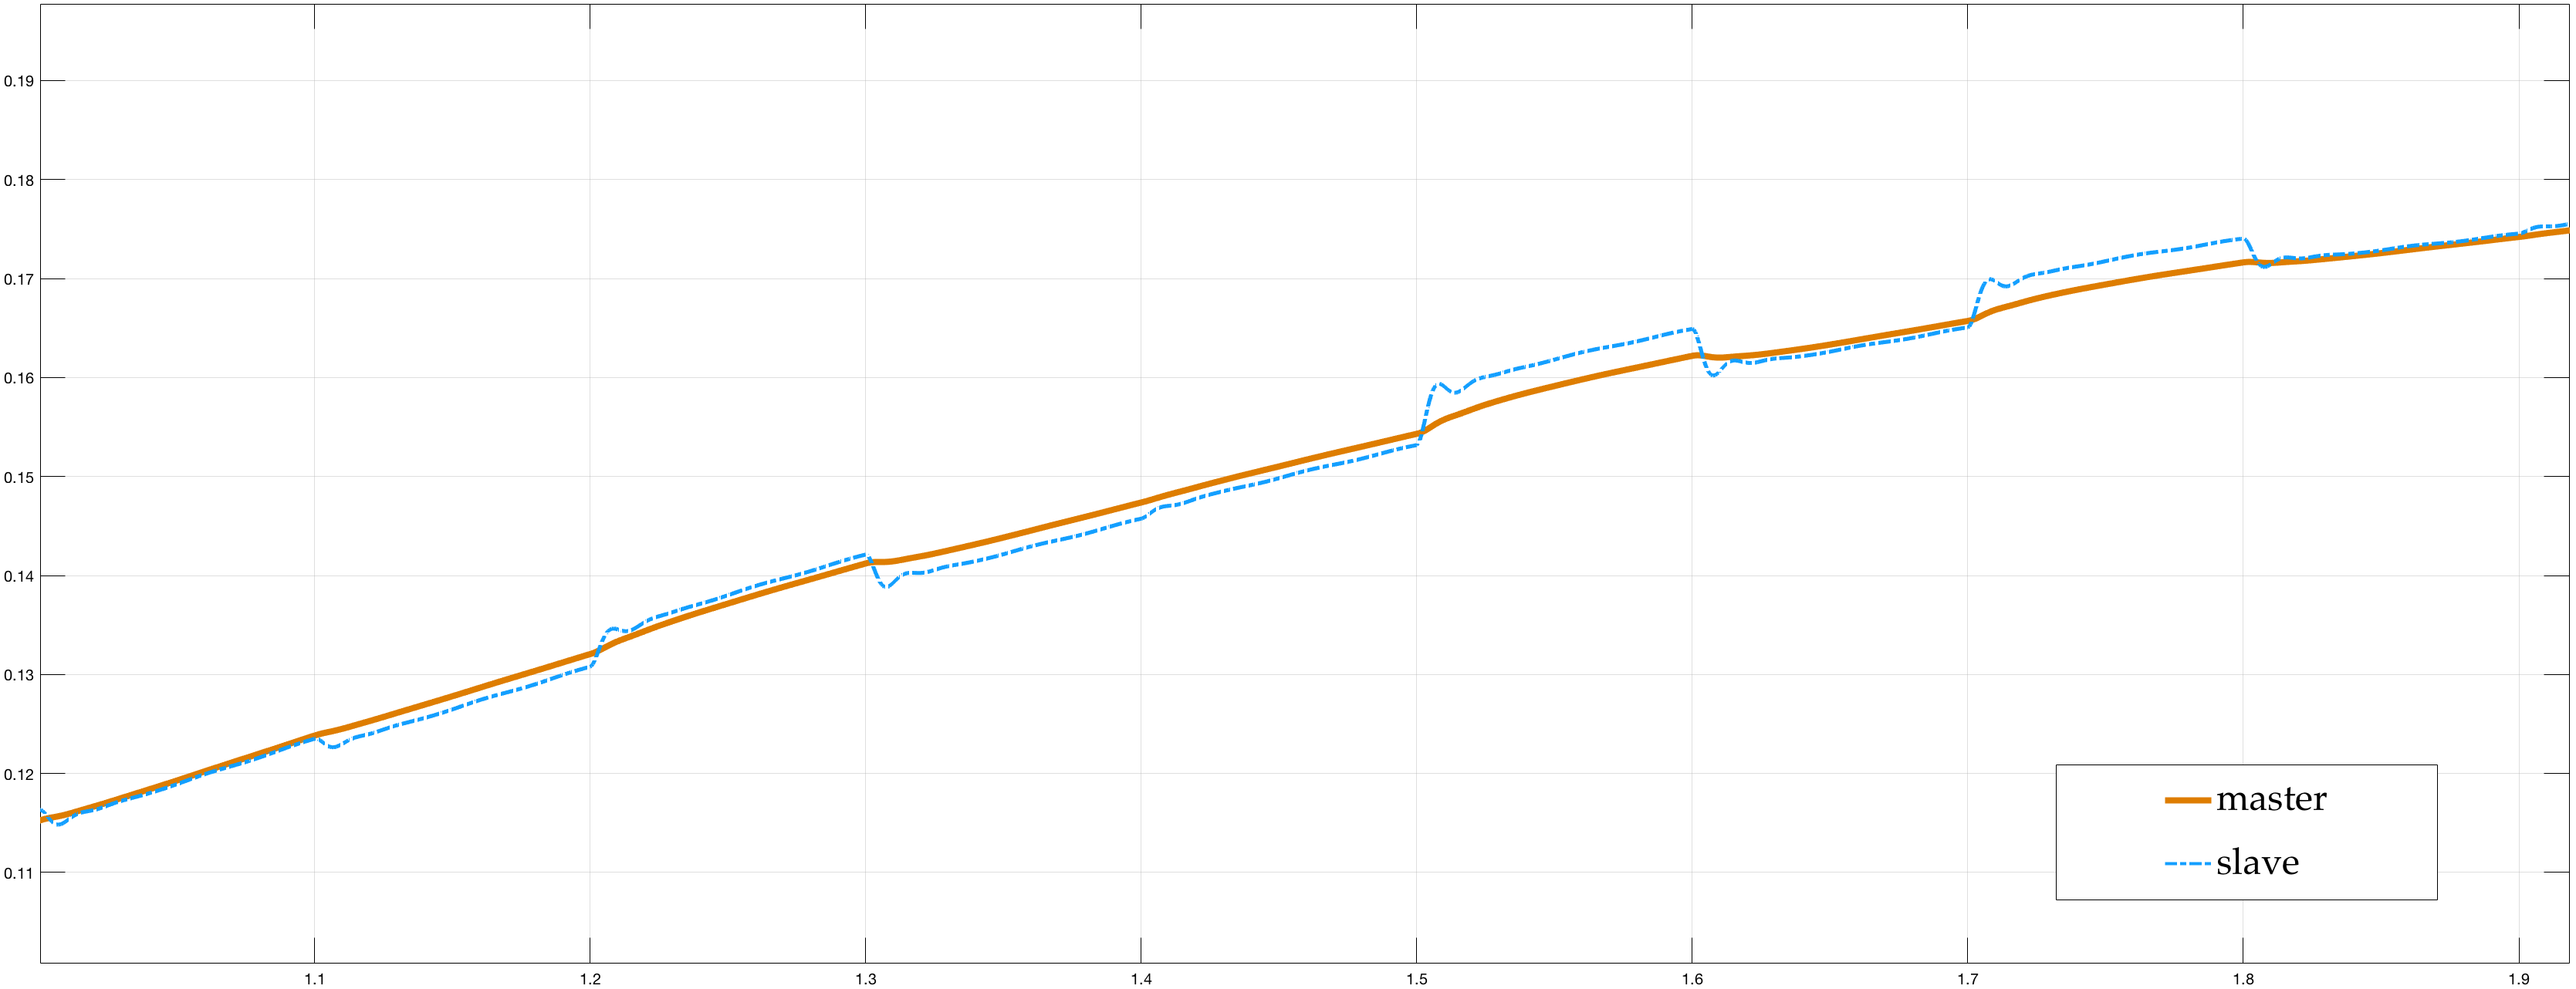
\includegraphics[width=\textwidth, height=0.48\textwidth]{Images/freerigidPart20Htznoise}
		\caption{Detail describing the highlighted area in fig.\ref{fig:freeRigTot20HR}}
		\label{fig:freeRigPar20HR}
	\end{subfigure}	
 \caption{\textbf{Low} frequency disturbances response - rigid coupling control.}
\end{figure}

This phenomenon shows up in fig.\ref{fig:freeRigPar20HR} and fig.\ref{fig:freeSetPar20HR}. Infact the two profiles confirm that \textsl{rigid coupling control} cancel out most of the useful information from the signal, while \textsl{virtual compliance control} saves the signal information.
%which is extremely important from a control perspective.

\subsubsection{Contact motion}

%In this section the proposed simulations hold the same reference trajectory for
%master than the simulations in free motion. 
In this section the reference trajectory for master is equal to the one used for the simulations in free motion.
%But, in addiction, after that the slave would trespass a certain angle value
%there would be a contact with the environment, this wouldn't allow a perfect
%tracking by the slave.

The slave, overcoming a certain angle value, is in contact with the environment. This will not allow a perfect tracking by the slave.

The comparison between \textsl{virtual compliance control} and \textsl{rigid coupling control} in presence of a contact with the environment can be deduced by the
differences in \textbf{magnitude} of the arrows drawn in the fig.\ref{fig:contact_virtual} and fig.\ref{fig:contact_rigid}.

\begin{figure}[H]
	\begin{subfigure}{1\linewidth}
		\centering
		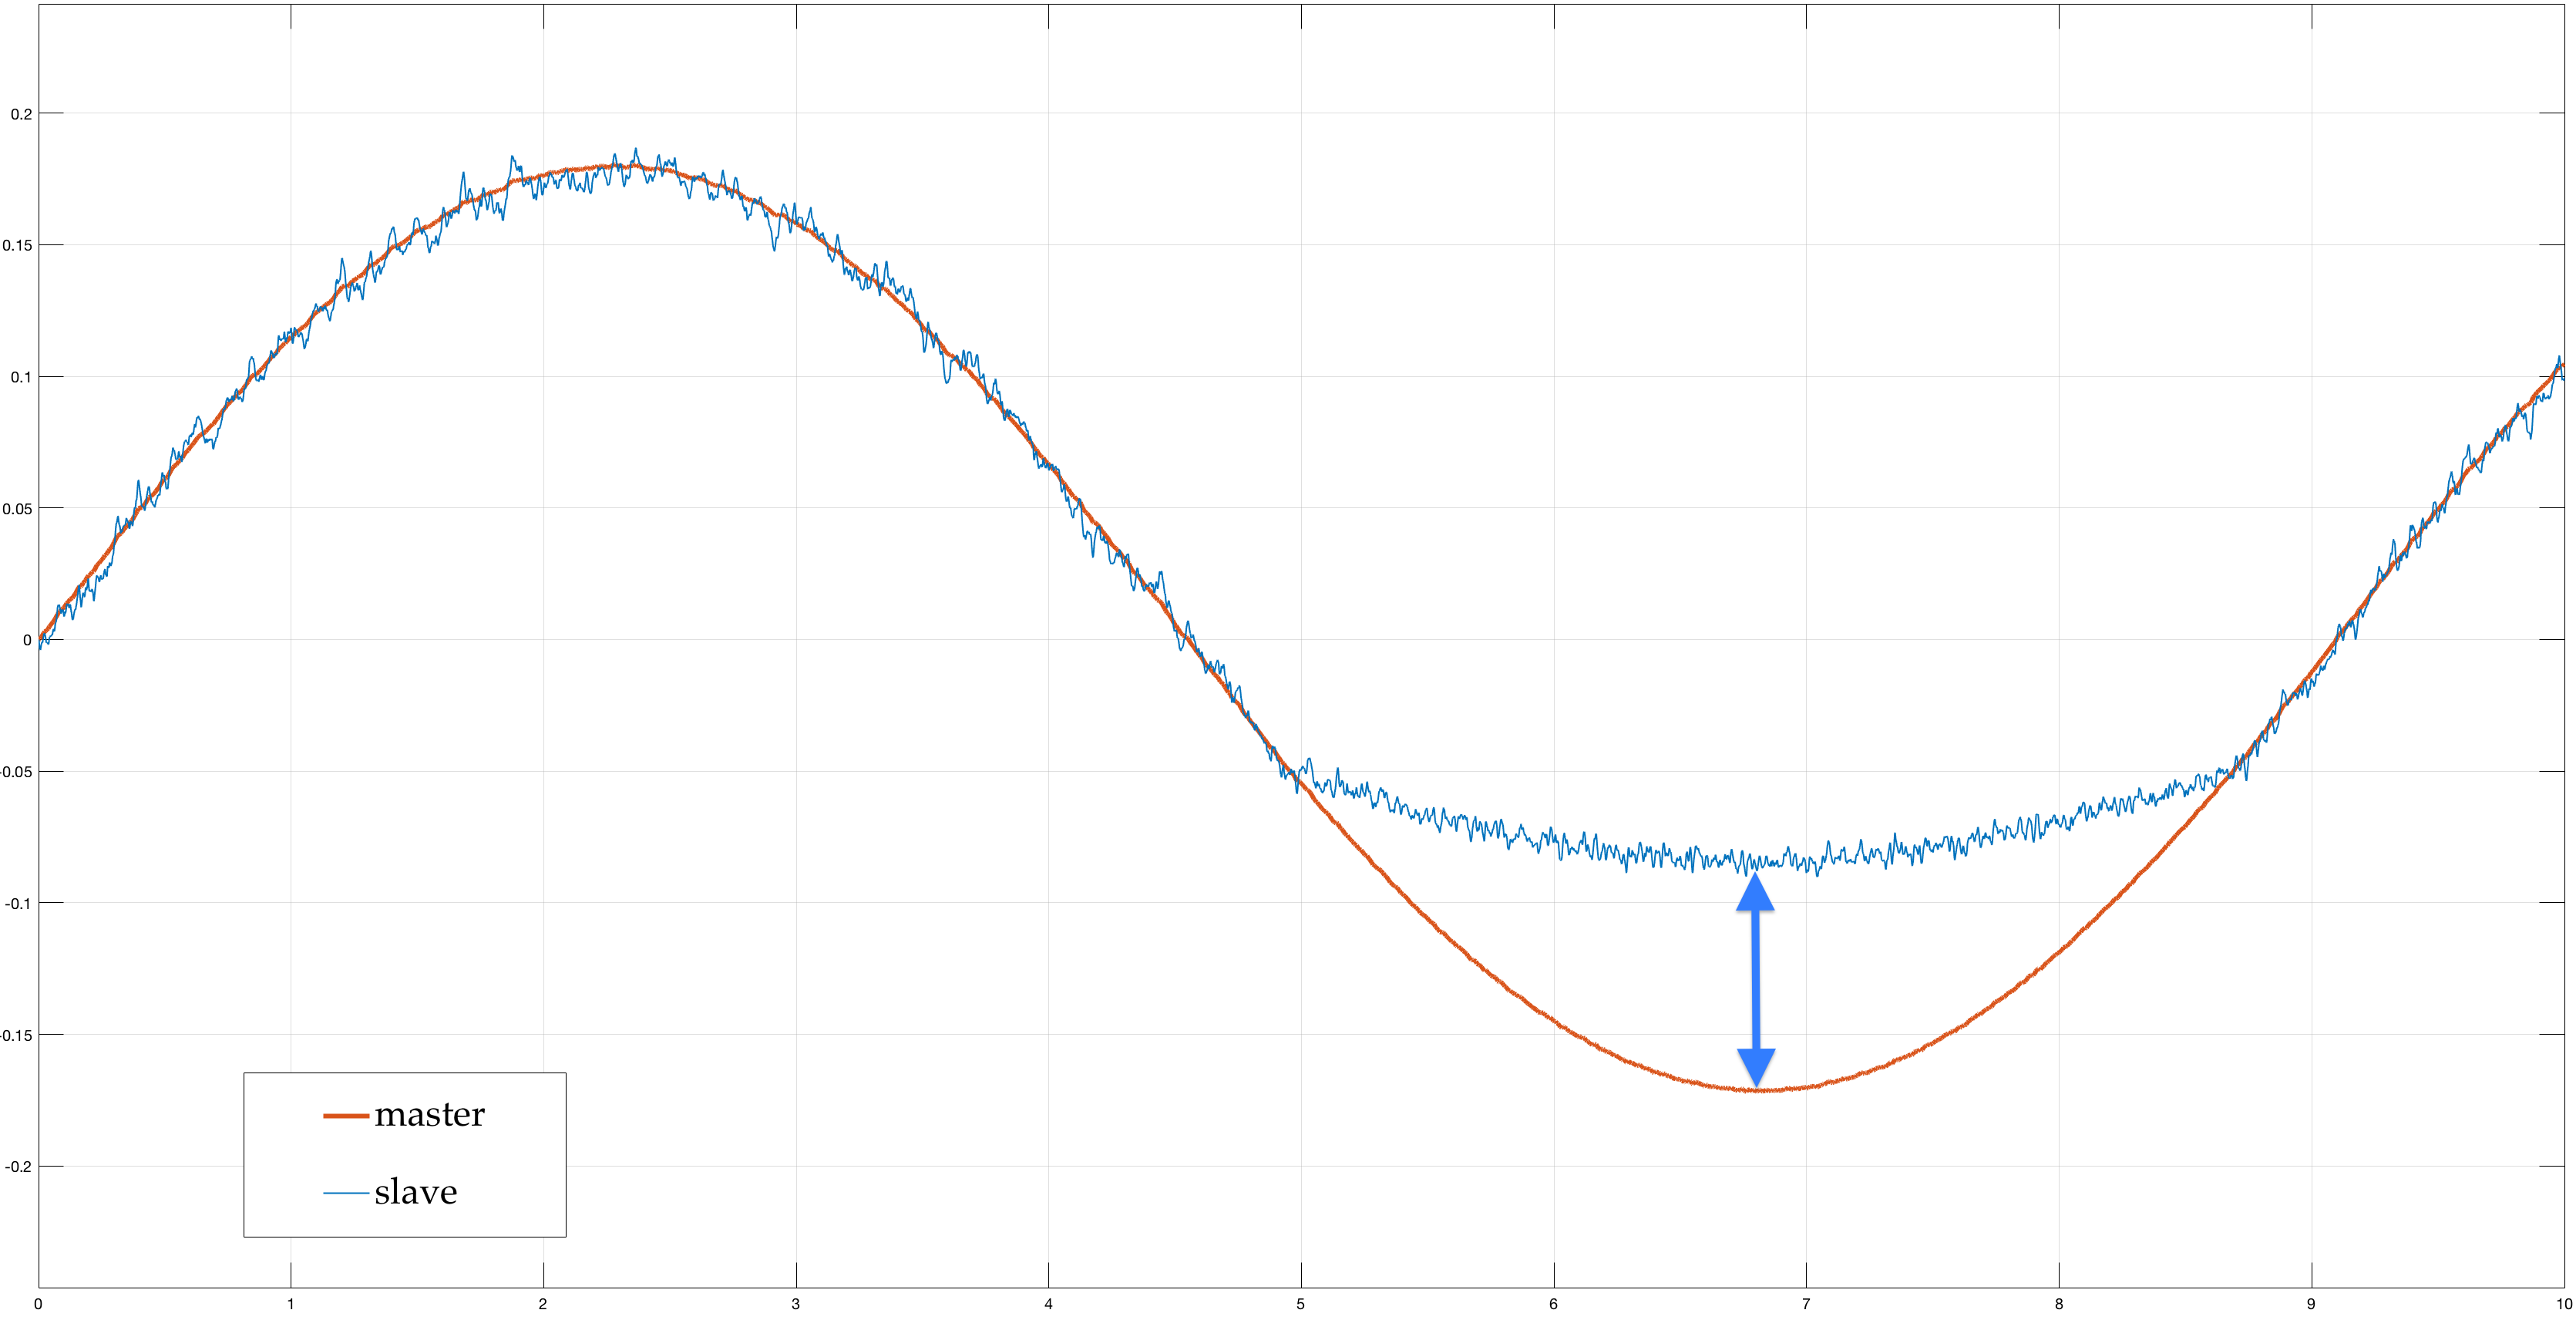
\includegraphics[width=\textwidth, height=0.41\textwidth]{Images/setPointContactReacPosArrow}
		\caption{Position assumed during trajectory tracking.}
		\label{fig:ContactSetPos}
	\end{subfigure}	
\end{figure}
\begin{figure}[H]\ContinuedFloat
	\begin{subfigure}{1\linewidth}
		\centering
		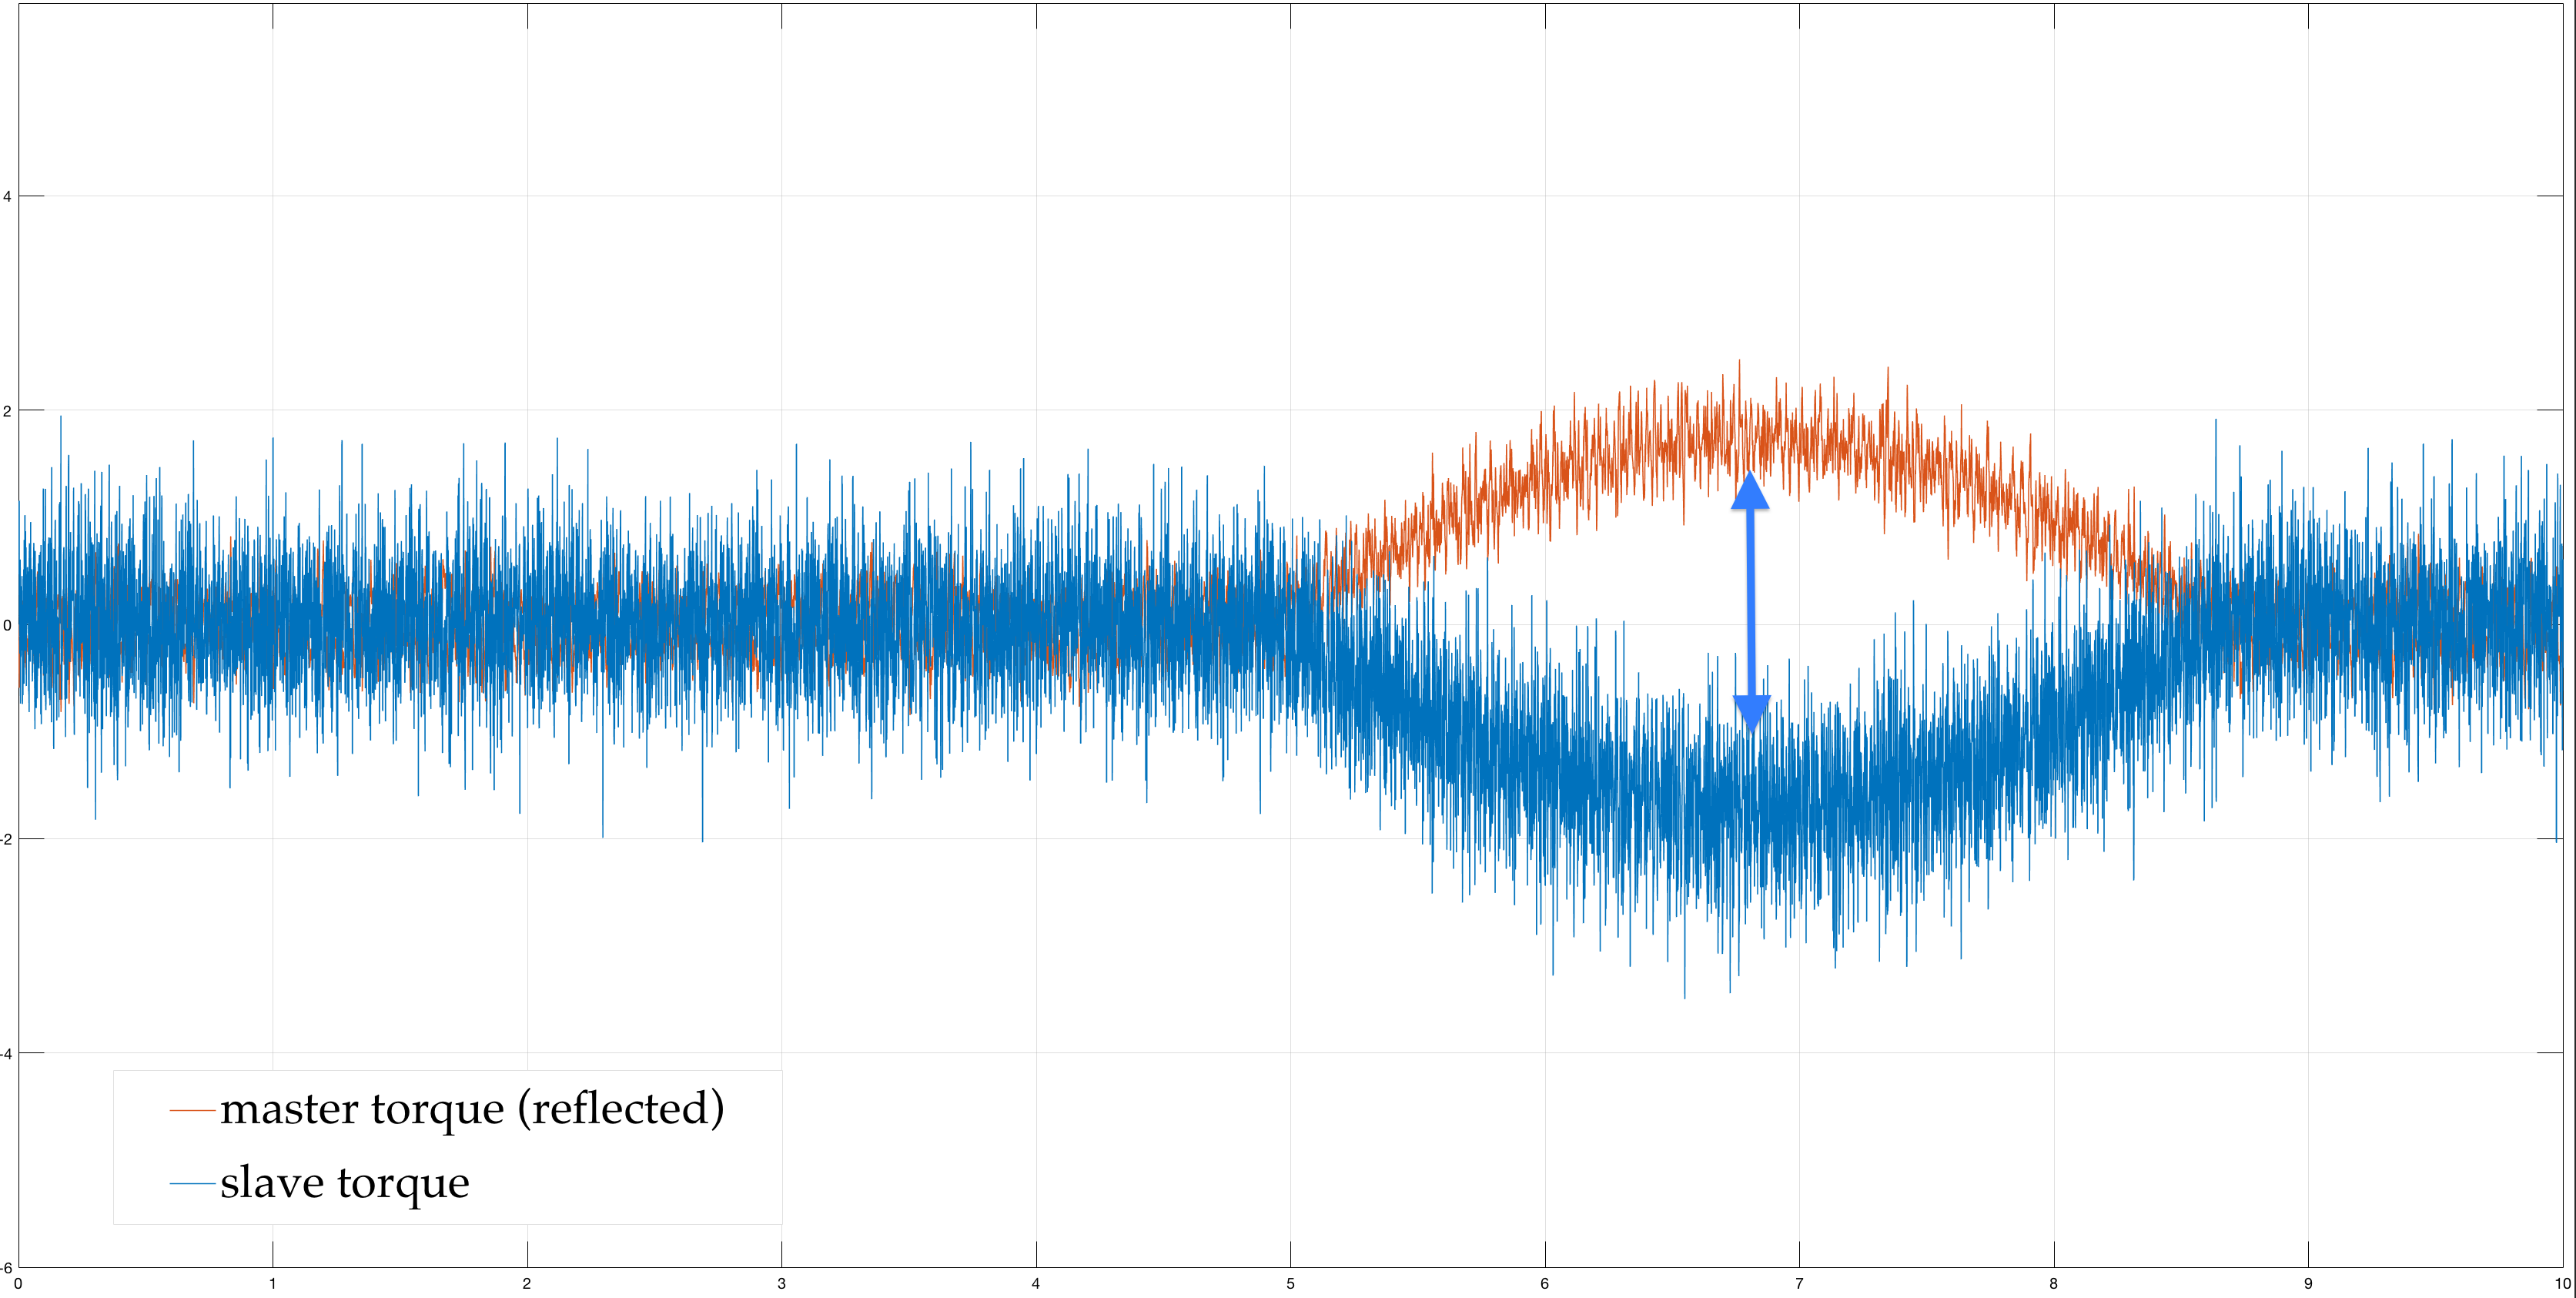
\includegraphics[width=\textwidth, height=0.41\textwidth]{Images/setPointContactReacTorArrow}
		\caption{Torques exerted over time.}
		\label{fig:ContactSetTor}
	\end{subfigure}	
 \caption{Contact motion simulation - virtual compliance control.}
 \label{fig:contact_virtual}
\end{figure}

%Concerning the position of slave with the respect of master the
%fig.\ref{fig:ContactSetPos} portraits a worse performance in trajectory error
%when in contact behaving in \textsl{virtual compliance} than behaving in
%\textsl{rigid coupling} (fig.\ref{fig:ContactRigPos}).

During the contact motion phase, a gap between the master and the slave position emerges. Fig.\ref{fig:ContactSetPos} shows as the \textit{virtual compliance control} leads to a larger position error then the \textit{rigid coupling control }(fig.\ref{fig:ContactRigPos}): with high spring stiffness value the gap is closer.

From the point of view of the torque exerted, the proposed control
(fig.\ref{fig:ContactSetTor}) performs more efficiently than \textsl{rigid coupling coupling} (fig.\ref{fig:ContactRigTor}), suppressing the high frequency noise from the environment to the master side.

  
\begin{figure}[H]
	\begin{subfigure}{1\linewidth}
		\centering
		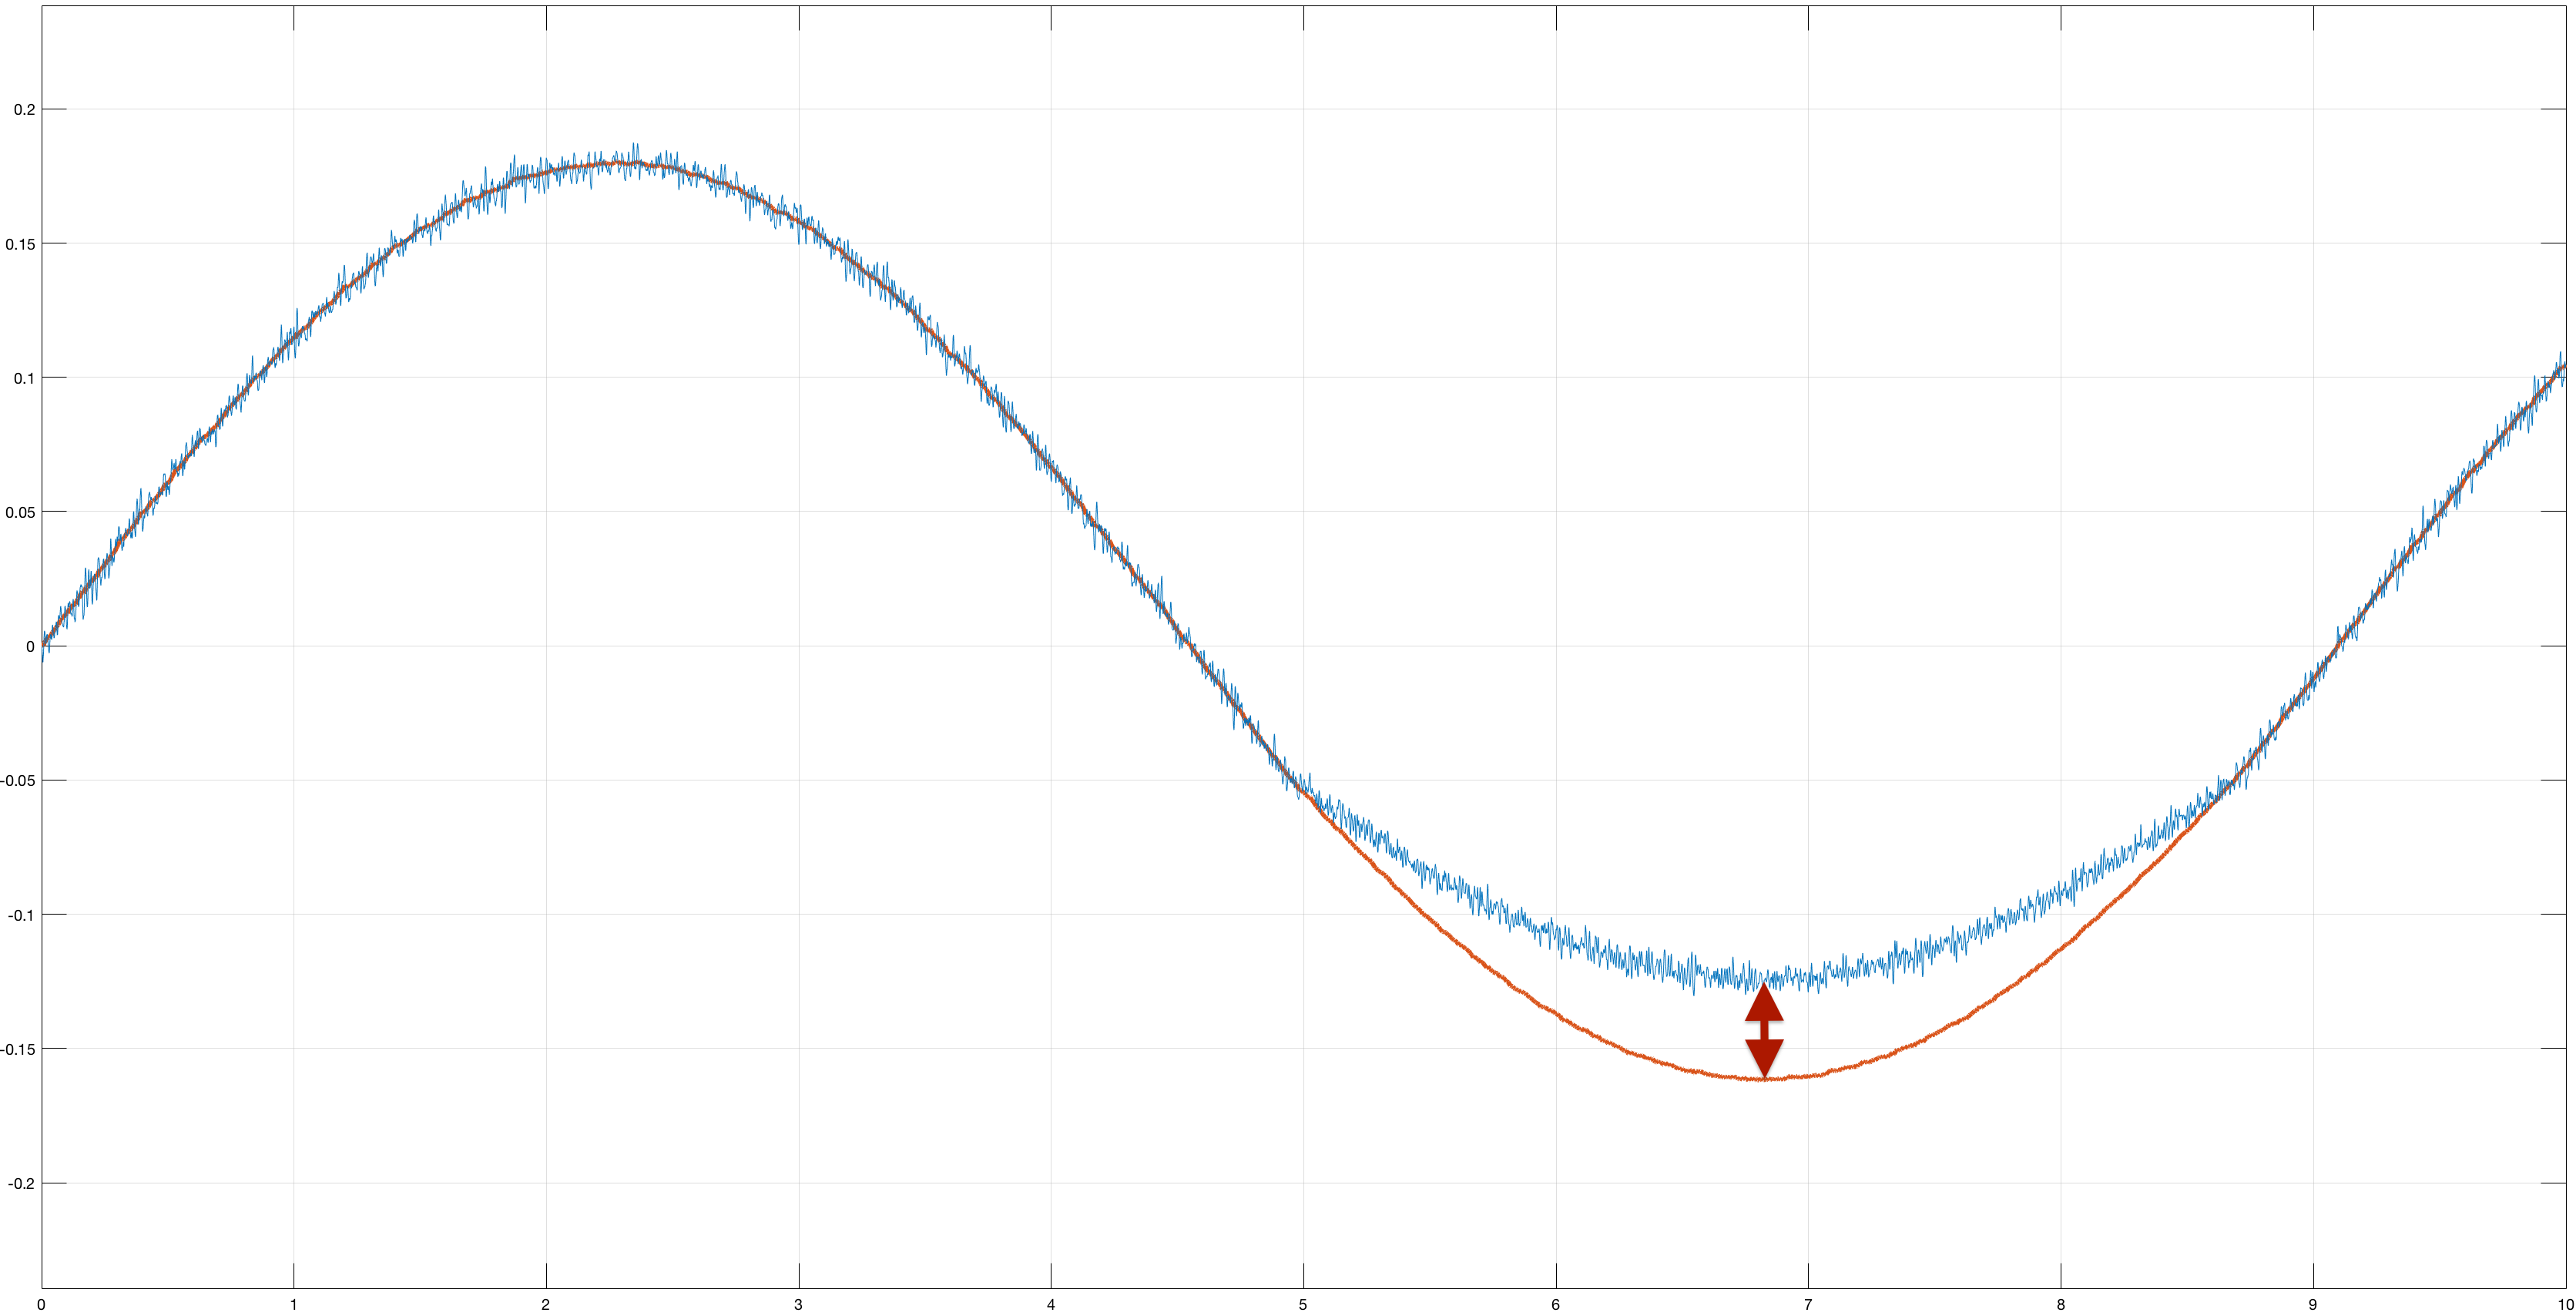
\includegraphics[width=\textwidth, height=0.41\textwidth]{Images/rigidContactReacPosArrow}
		\caption{ Angular position assumed during trajectory tracking.}
		\label{fig:ContactRigPos}
	\end{subfigure}	
\end{figure}
\begin{figure}[H]\ContinuedFloat
	\begin{subfigure}{1\linewidth}
		\centering
		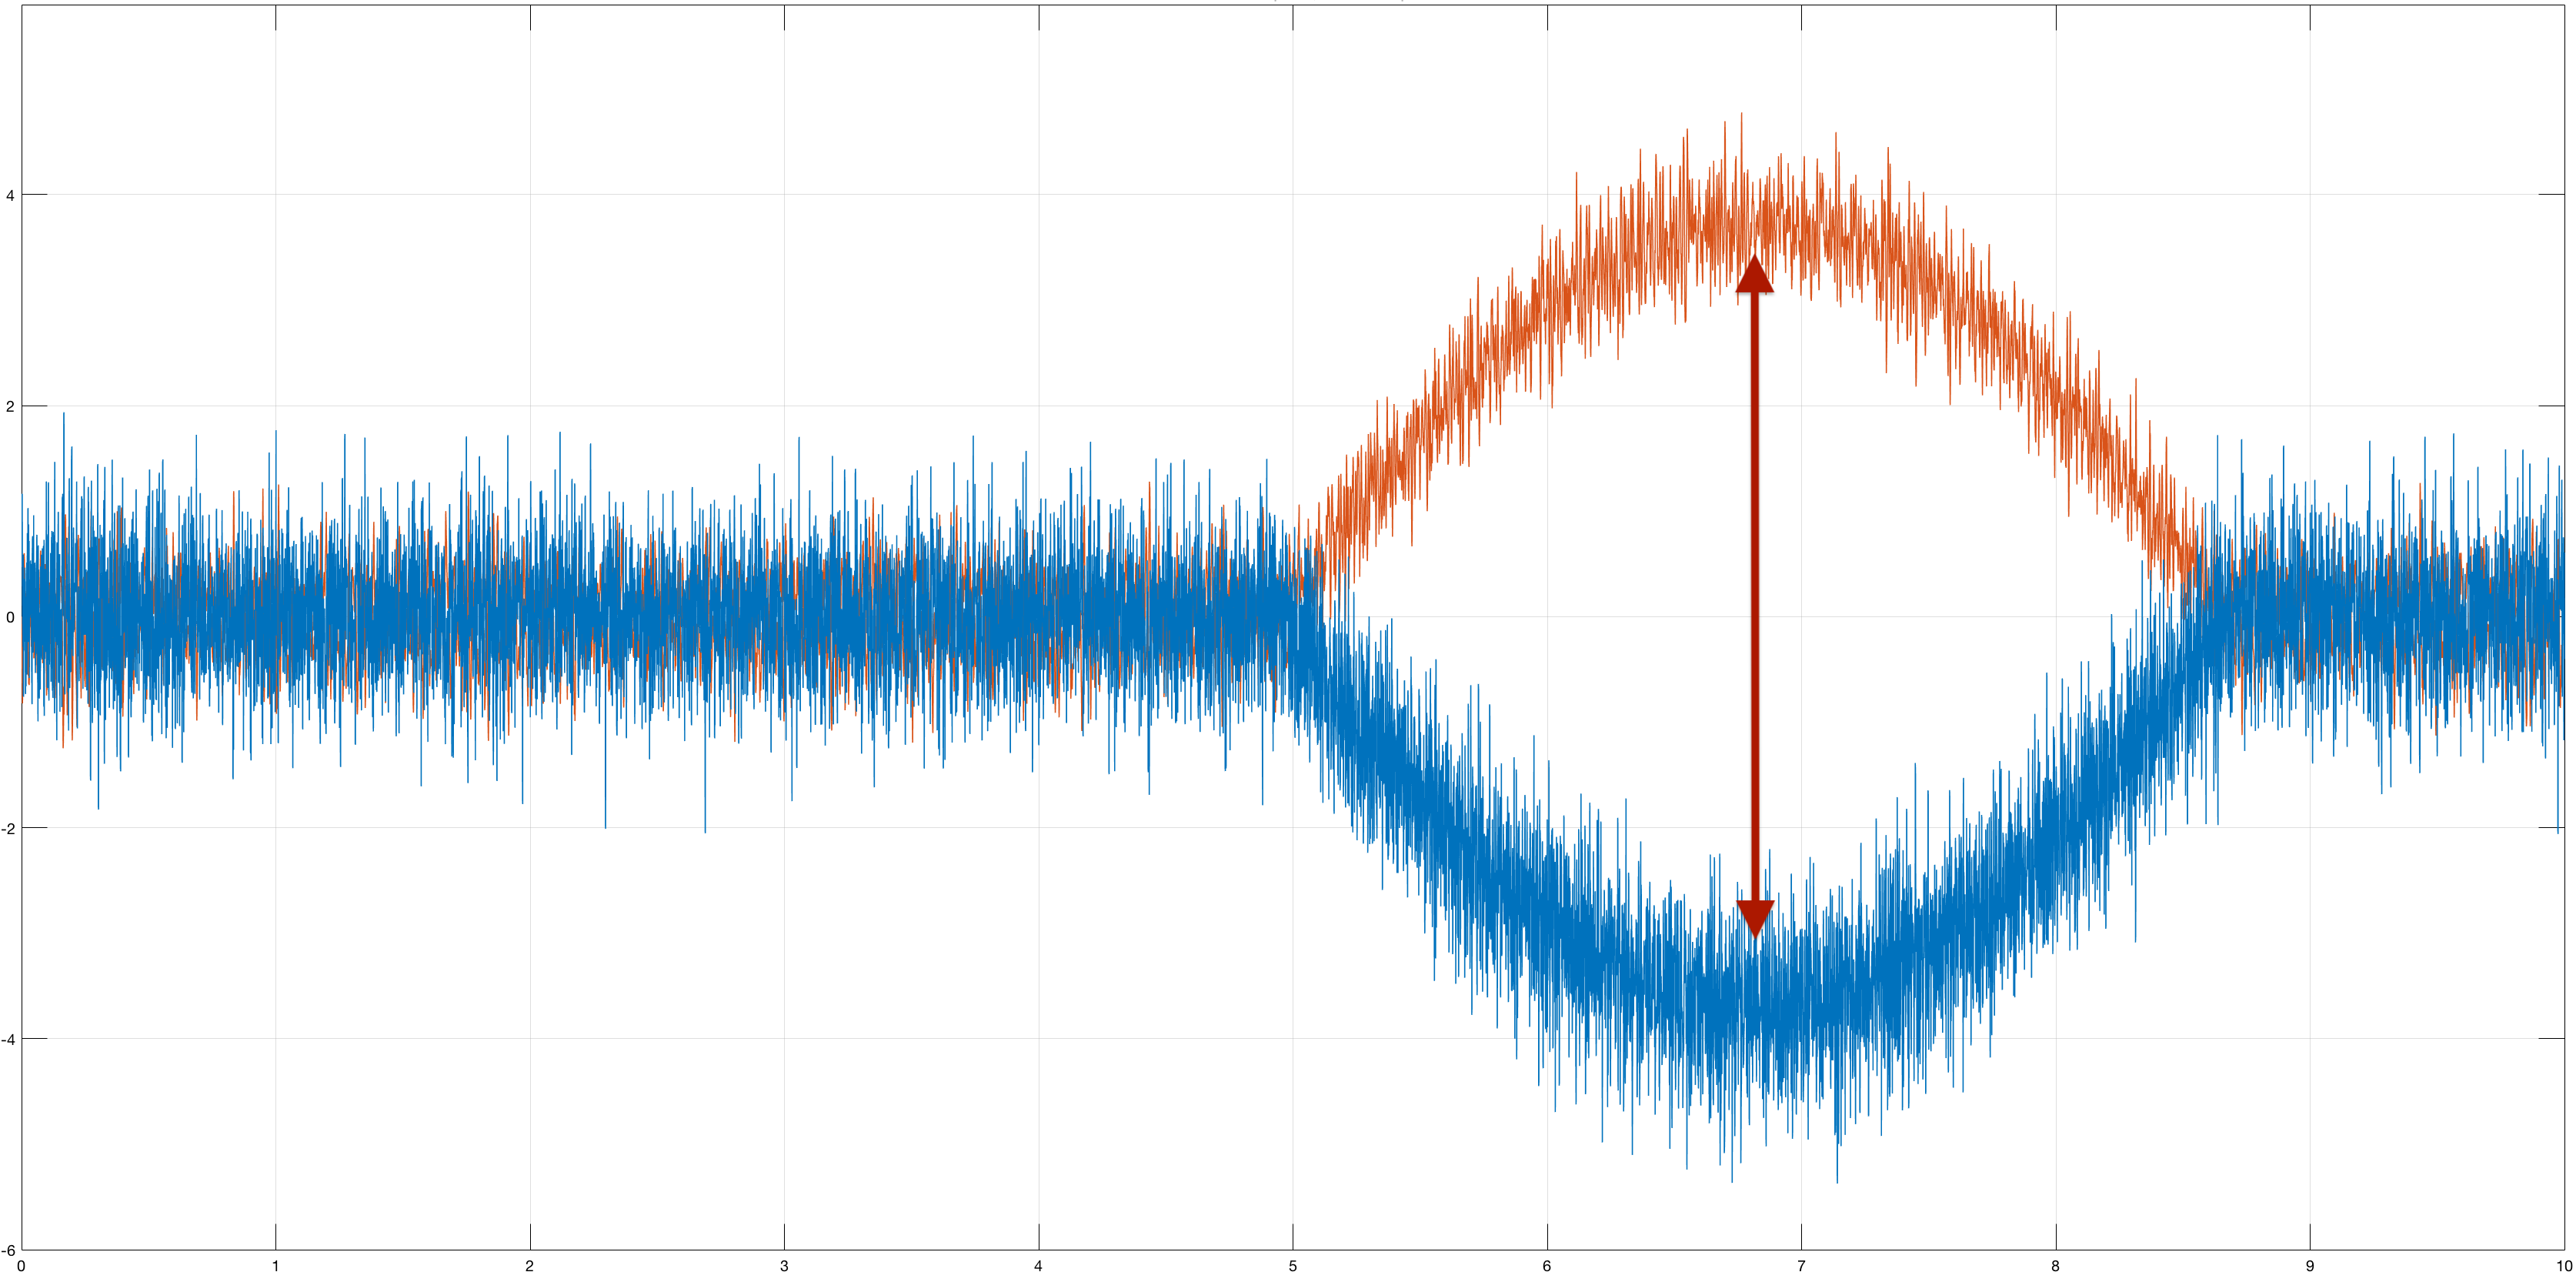
\includegraphics[width=\textwidth, height=0.41\textwidth]{Images/rigidContactReacTorArrow}
		\caption{ Torques exerted over time}
		\label{fig:ContactRigTor}
	\end{subfigure}	
  \caption{ Rigid coupling simulation in \textsl{contact} with the environment}
  \label{fig:contact_rigid}
\end{figure}

\newpage

\section{Conclusions}
Vibration suppression in the contest of bilateral teleoperation is an open
issue.
\bigskip

The proposed solution is based on a virtual spring-damper system with additional
inertia. The spring stiffness and the cut-off frequencies are chosen according to the system requirements.
\bigskip

To summarize, when the virtual stiffness has been fixed, the other virtual
parameters could be calculated from the equations in order to obtain the desired
cut-off frequencies.
\bigskip

The tracking error in \textit{free motion} is almost the same, using both \textbf{virtual compliance control} and \textbf{rigid coupling control}. However,the proposed controller shows promising results, since it preserves the useful (\textsl{low}) frequency inputs and reject the noisy ones (\textsl{high}). 
\bigskip
%Overall, the tracking error in free motion is almost null. And regarding the contact with the environment is interesting to observe from the simulations a trade-off between control effort and task error.

In \textit{contact motion} the usage of the proposed controller leads to a position gap between master and slave and hence can be applied only to tasks that involve the handling of \textsl{soft} materials.



	

\appendix

\end{document}
